\chapter{METHODOLOGY}

\section{Methodology}\label{ch:Methodology}

\hspace{12pt} In our methodology, we begin by considering the overarching scenario of the \ac{EEWs}. This system comprises numerous earthquake detectors positioned randomly in various locations such as households, offices, and other relevant settings. These detectors continually operate to identify seismic activity. When an earthquake detector detects and verifies a seismic wave, we refer to this as a detection point. In the event of a seismic wave detection, we assume its impact to be consistent across all points within a 30 km radius from the detection point. Therefore, our objective is to transmit a warning message beyond this 30 km radius circular area around the detection point within 10 seconds (The arrival time of S waves at a point 30 km away). Our communication architecture is specifically designed with a focus on minimizing latency since the effectiveness of the warning messages hinges on their reception before the seismic wave arrives. We consider the detection of earthquakes from the S-wave, which propagates at approximately 3 km/s.\\

\subsection{Multi hop communication Setup}
\label{sec:multihop}
\hspace{12pt} Given our focus on achieving a 30 km range, it's important to note that accomplishing this distance with a single hop, even with the highest \ac{SF}, is not feasible without a line of sight. As outlined in \autoref{sec:Research}, \cite{farooq} suggests that employing three hops of the lowest \ac{SF} (SF7) can yield a comparable range to that achieved with the highest \ac{SF} (SF12), while also resulting in lower latencies. In our investigation, we sought to substantiate this concept through a combination of simulation and physical testing. Through an integration of simulation modeling and real-world experimentation, we successfully demonstrated significant time reductions.\\

The detailed numerical analysis supporting this finding, derived from the simulation, is presented in \autoref{ch:multihop_evaluation} of this document.\\

Observing the considerable reduction in time, we have chosen to integrate this concept into our methodology. Consequently, our approach revolves around the fundamental principle of utilizing multi-hops with lower \ac{SF}s to attain minimal latencies, instead of relying on higher \ac{SF}s.

\begin{figure}[htp!]
    \centering
    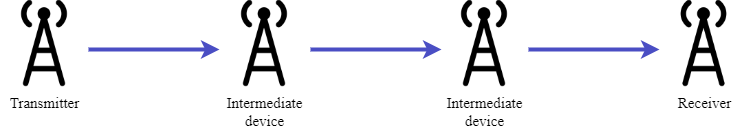
\includegraphics[scale=0.5]{images/simple_multihop.png}
    \caption{Simple Multi-hop Link }
    \label{fig:simple_multihop}
\end{figure}

\subsection{Proposed Architecture}
\label{sec:architecture}
\hspace{12pt} Our proposed architecture is based on the multihop concept, which is detailed in \autoref{sec:multihop}. This architecture diverges from the traditional LoRaWAN network topology. While LoRaWAN typically operates in a star-of-stars configuration, utilizing gateways as intermediaries between end devices and a central network server, our approach necessitates a departure from this standard.\\

The LoRaWAN MAC protocol imposes strict limitations, constraining channel usage to a mere 1$\%$ duty cycle per cycle, as mandated by regulatory authorities. Additionally, LoRaWAN enforces fair use policies. Given these constraints, a conventional LoRaWAN setup would not meet our requirements, particularly concerning latency optimization.\\

In response to our objectives, we have formulated a customized broadcast LoRa mesh network. A notable feature of our network architecture is the absence of routing mechanisms. Instead, devices broadcast packets indiscriminately, allowing any devices within range to receive the packets. By avoiding routing protocols, we mitigate potential time overheads that routing may introduce to our network. This streamlined approach ensures efficient and timely dissemination of critical information within our network.\\

Our communication system primarily comprises two types of devices: \textbf{End Nodes} and \textbf{Relay Nodes}. Below, we elaborate on the roles and distinctions between these device types. Additionally, a comparison of the two device types is provided in \autoref{tab:comparison_of_devices}.\\

\noindent\textbf{End Devices:}\\

These units serve as the interface directly with earthquake detectors. Operating in an always-on mode, the end nodes continuously monitor for incoming packets. Upon detecting seismic activity, the earthquake detector signals the connected end device, prompting it to generate an earthquake warning message. Subsequently, the end device functions as the transmitter, broadcasting this warning message. However, it's important to note that not all end nodes are necessarily connected to earthquake detectors; some end nodes may function solely as receivers. Additionally, regardless of their connection to earthquake detectors, end nodes are expected to be integrated with the alerting system, which may include an alarm or similar mechanism.\\

During a single occurrence, only the end node connected to the earthquake detector transmits messages; however, all other end nodes remain on standby, ready to receive incoming warning messages. Upon receiving a warning message, the alerting system connected to the end node, typically an alarm, is activated, initiating the alert process.\\

The location and density of end devices are unrestricted. Our primary focus is to establish a crowd-sourced \ac{EEWs} capable of accommodating the integration of new end nodes over time.\\

\noindent\textbf{Relays:}\\

These devices play a critical role in the Earthquake Early Warning System (EEWS). They can be identified as a customized type of gateway specifically designed for our communication setup. Their primary responsibility is to receive messages from either end nodes, particularly the one connected to the detection point, or other relay nodes. Upon receiving a message, relay nodes broadcast the warning to all connected devices. However, their duty concludes after broadcasting the warning message. Although relay nodes may continue to receive messages after broadcasting, they do not re-broadcast the same warning message repeatedly.\\

The placement of relay nodes is strategically predetermined to ensure optimal coverage of the entire area where the EEWS is implemented. This strategic positioning guarantees that all end nodes within the system, as well as those that may be added in the future, are adequately covered. Accordingly, relay nodes are strategically positioned to optimize both the lowest density and minimize collisions, ensuring efficient data transmission throughout the entire area.\\

It is indeed crucial to note that relay nodes may sometimes interface with the alerting systems as well. Additionally, in certain scenarios, relay nodes may also be connected directly to earthquake detectors. However, it's important to emphasize that the placement of relay nodes is strategically predetermined and cannot be changed once installed.

\begin{table}[htp!]
\begin{tabular}{|l|l|l|}
\hline
\multicolumn{1}{|c|}{Feature} & \multicolumn{1}{c|}{End Nodes} & \multicolumn{1}{c|}{Relay Nodes} \\ \hline
Operation mode   & Always on               & Always on          \\ \hline
Device density                & Can be changed over time       & Fixed number of devices          \\ \hline
Device placement & Unrestricted            & Predetermined       \\ \hline
Role             & Transmitter or Receiver & Customized gateway \\ \hline
\end{tabular}%
\caption{Comparison of End Nodes and Relays}
\label{tab:comparison_of_devices}
\end{table}

\noindent\textbf{Proposing a Generalized Architecture:}\\

Given the crowd-sourced nature of our \ac{EEWs}, designing the architecture for specific node placements becomes impractical. Thus, we opt for a generalized scenario outlined as follows:\\

\noindent\textbf{End Node Distribution:} End nodes are randomly distributed within a circular region, following a uniform distribution. This approach ensures that the system will operate effectively regardless of the placement of individual end nodes in our crowd-sourced system.\\

\noindent\textbf{Relay Node Distribution:} Relay nodes are strategically positioned at predetermined locations, also uniformly distributed. The positioning of relay nodes has been optimized after experimenting with various positioning schemes, as further discussed in \autoref{ch:relays}.\\

In our generalized scenario, we position end nodes and relay nodes as described above. Subsequently, we select an end node as the detection point and consider a circular area of 30 km around it. Within this area, our objective is to transmit warning messages before the arrival of seismic waves. The generalized architecture is depicted in \autoref{fig:general_architecture}, providing a visual representation of the system's components.\\

\begin{figure}[ht!]
    \centering
    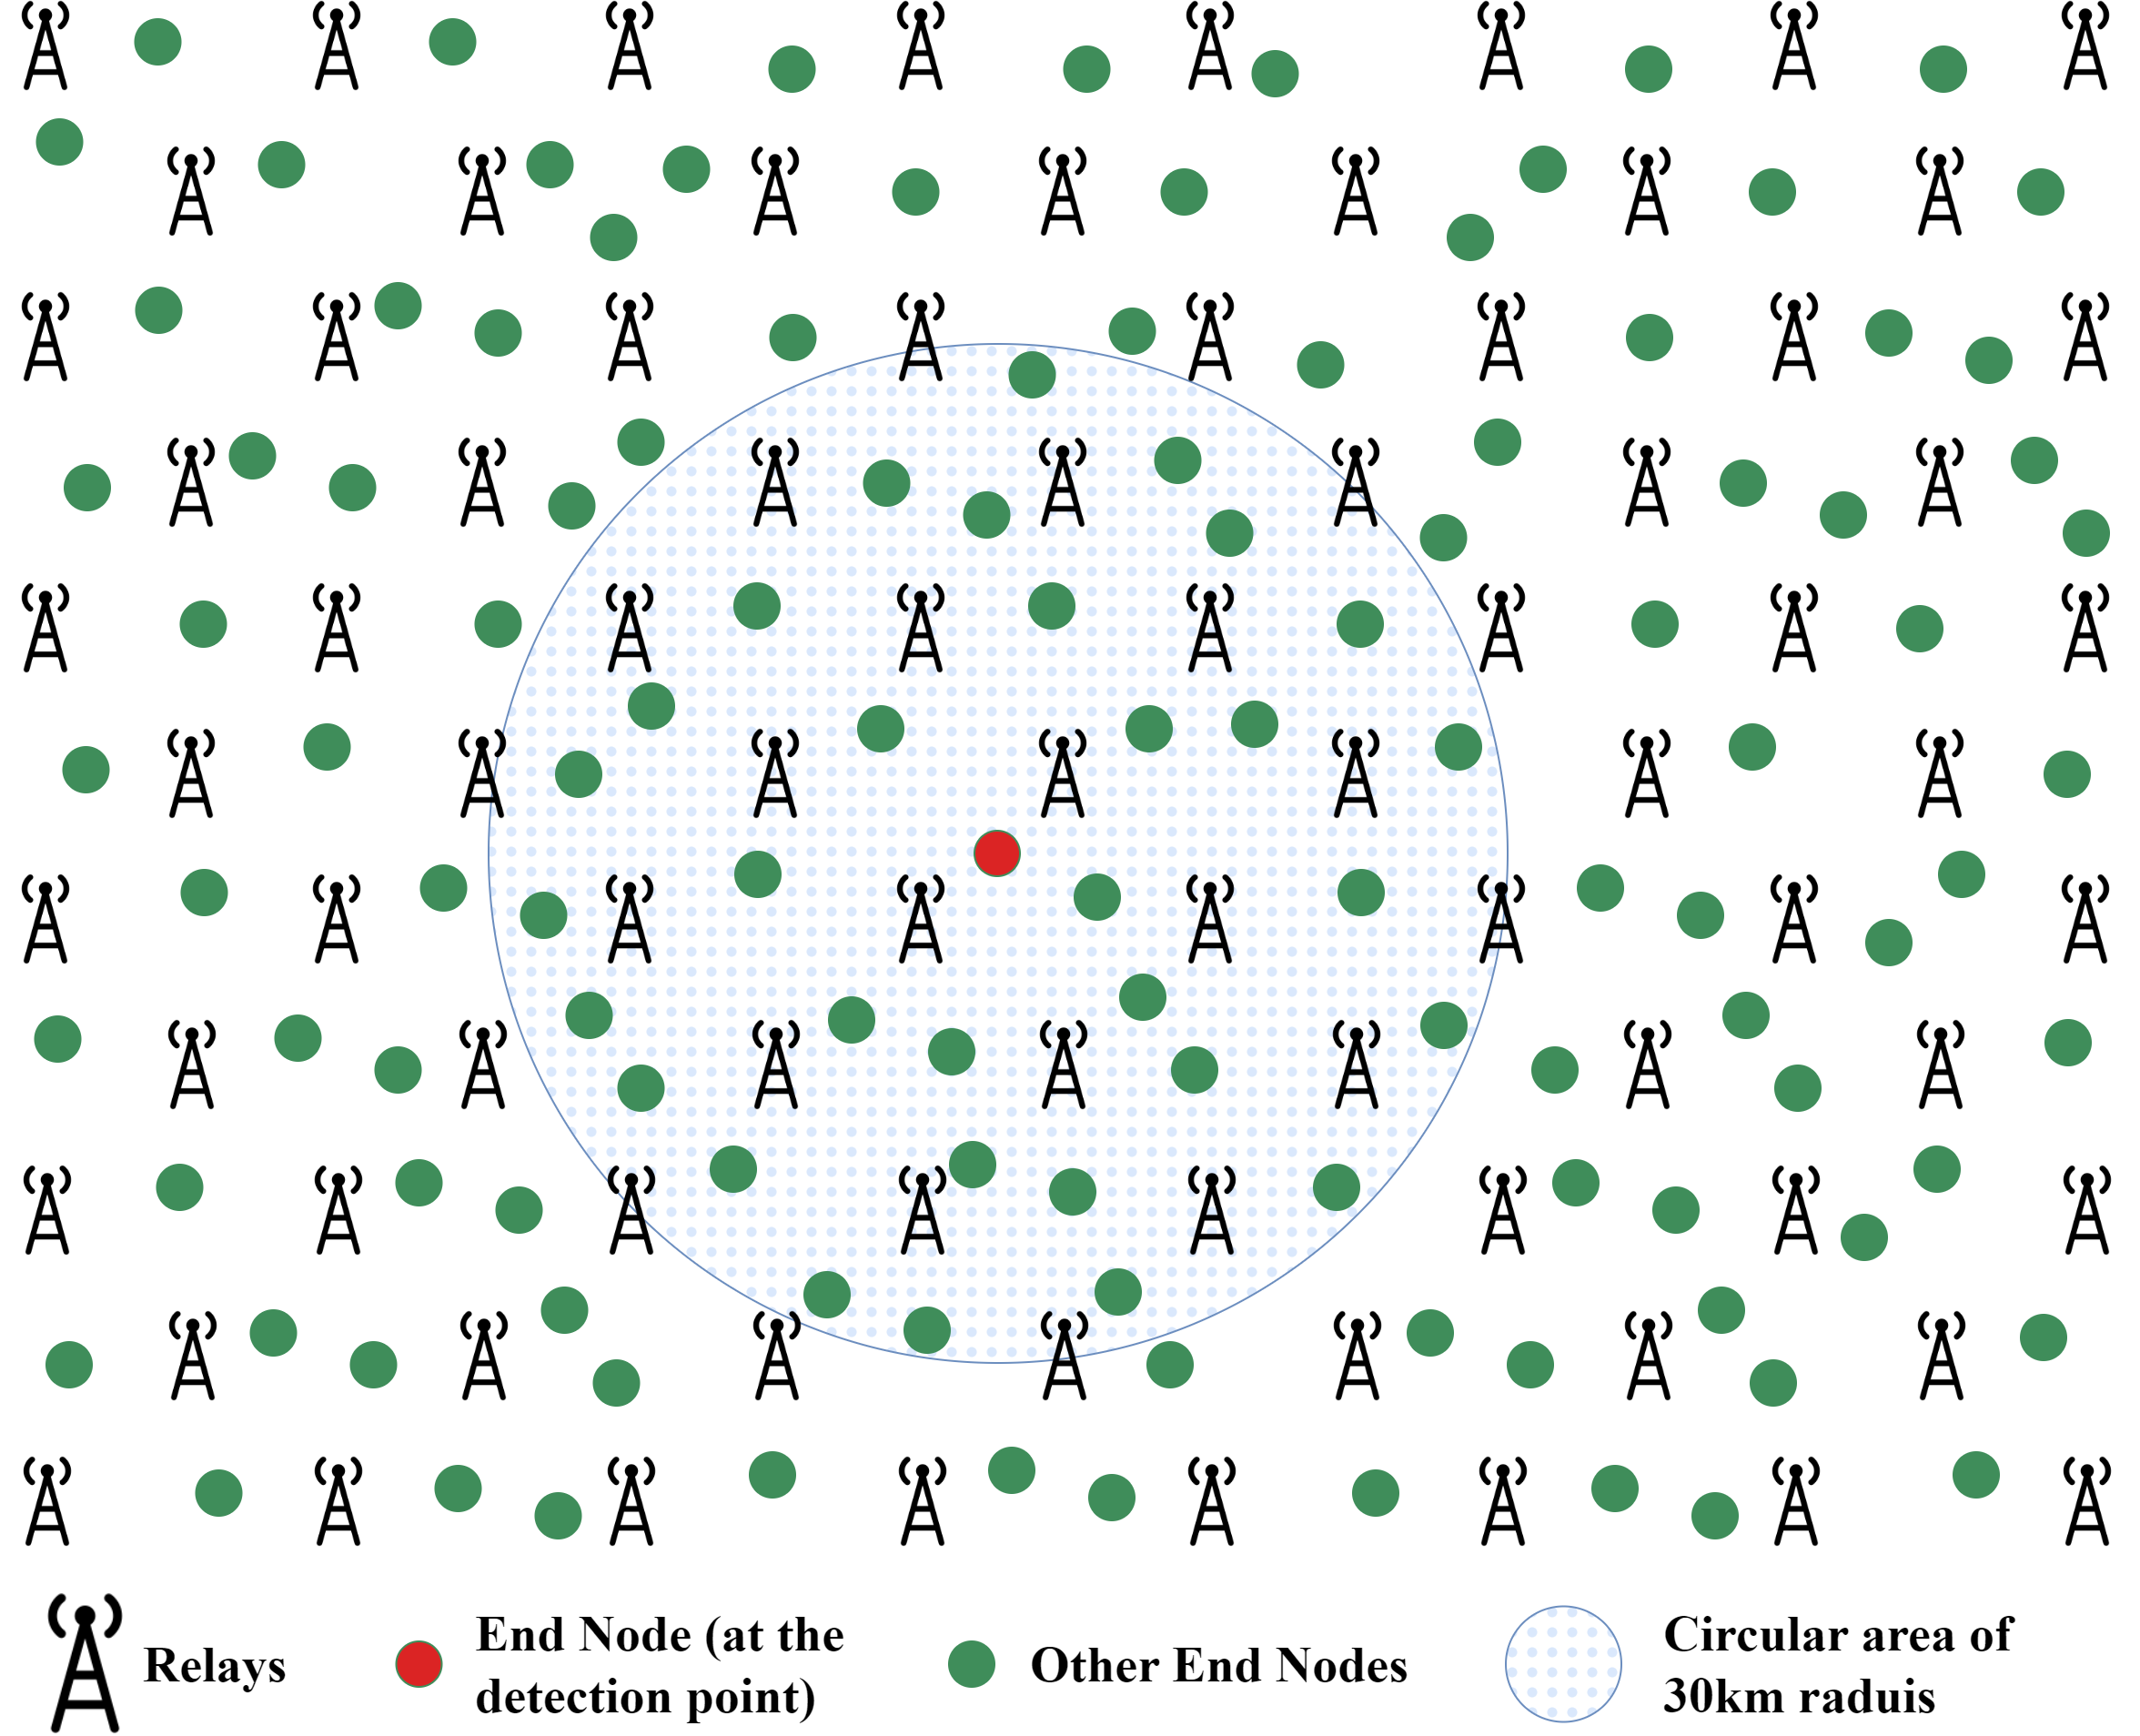
\includegraphics[width=0.8\linewidth]{images/generalarchitecture.png}
    \caption{Generalized Architecture}
    \label{fig:general_architecture}
\end{figure}

%------------------------------------------------------------------------------------------
\section{Device Selection}\label{ch:device}

\hspace{12pt} In order to verify the hardware configurations and test the communication system in a real-world scenario, we chose a pre-existing portable device built using ESP32 boards.
% \begin{figure}[ht!]
%     \centering
%     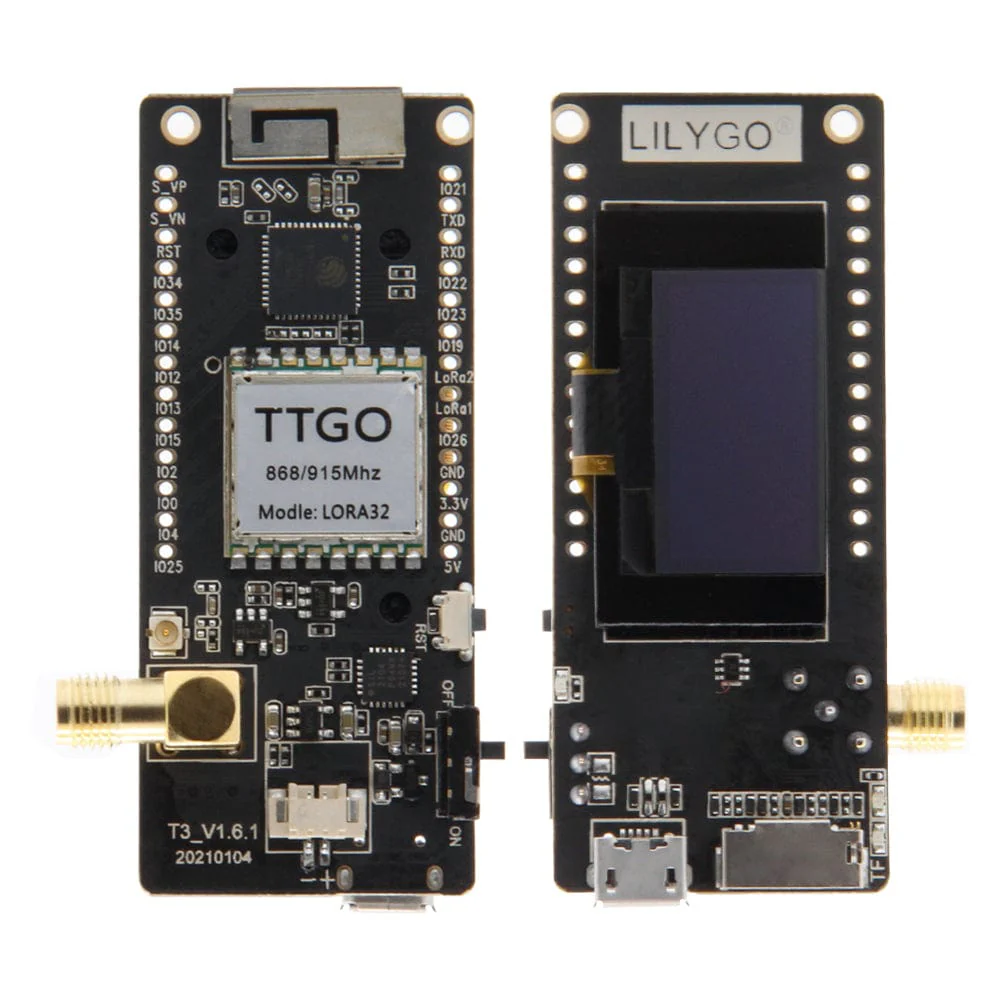
\includegraphics[width=0.5\linewidth]{images/lilygo.png}
%     \caption{LoRa32 V2.1\_1.6}
% \end{figure}

\begin{figure}[ht!]
    \centering
    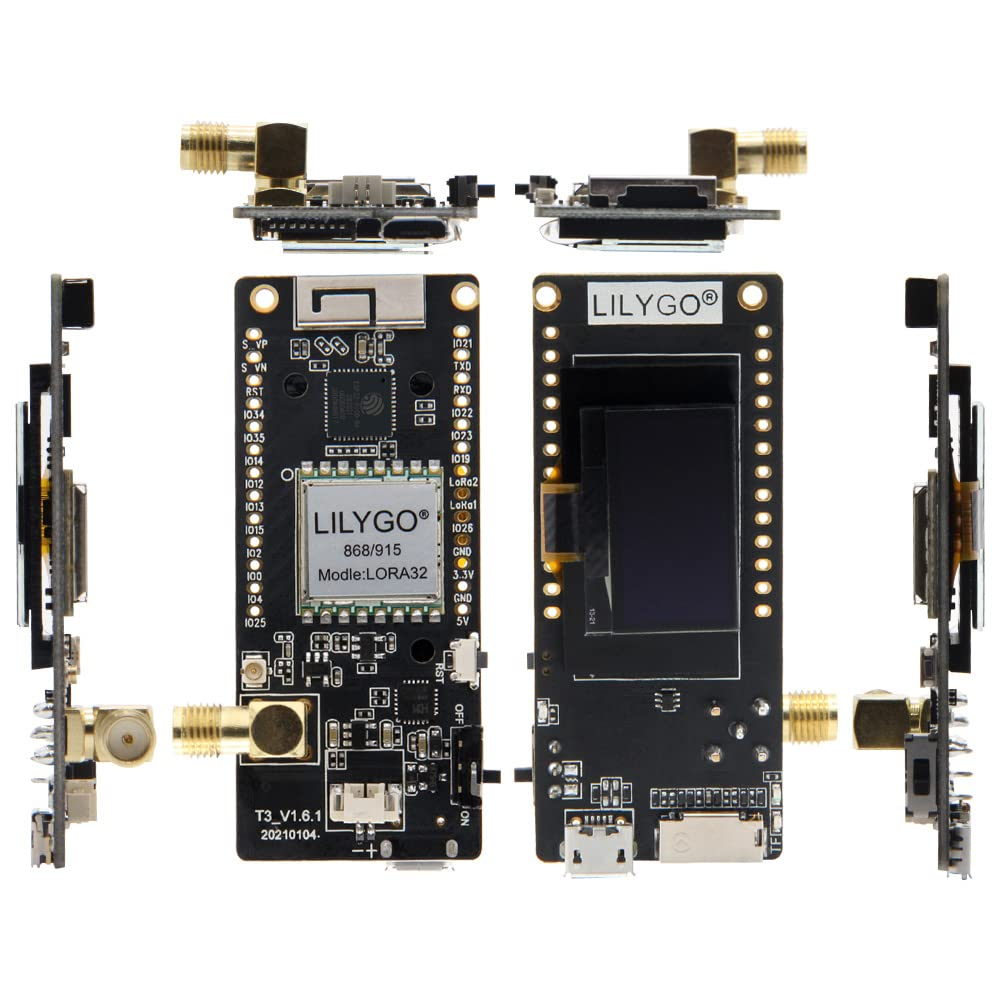
\includegraphics[width=0.5\linewidth]{images/lilygo_2.png}
    \caption{LoRa32 V2.1\_1.6}
\end{figure}


\begin{table}[ht!]
% \centering
\begin{tabular}{|l|l|}
\hline
\textbf{Parameter}                                                   & \textbf{Value}    \\ \hline
Microcontoller                                                       & ESP32             \\ \hline
\begin{tabular}[c]{@{}l@{}}Operating frequency\\ (LoRa)\end{tabular} & 923MHz            \\ \hline
LoRa Chip                                                            & SX1276            \\ \hline
Tx power                                                             & 2-17 dBm \& 20dBm \\ \hline
\end{tabular}
\caption{Lilygo LoRa32}

\end{table}

The SMA omini-directional 2dBi antennas are included with the devices, which also support WiFi and Bluetooth functions. These devices also have a convenient OLED display and the option to utilize an SD card interface.\\

The Lilygo LoRa32 device is ideal for our experiments given its low price point of around 17 USD and compatibility with various Libraries with Sx1276 Chip. We also came across a plethora of use cases for this device in the literature which further affirmed our decision.

%------------------------------------------------------------------------------------------
\section{Simulation Tool Selection}\label{ch:simulation}

\subsection{Selection Process}
\label{sec:simulation-selection}
% comparison of simulation tools
\hspace{12pt} Given that our research explores a non-conventional approach, necessitating numerous logical alterations within a typical LoRa and LoRaWAN network, the simulation software chosen plays a crucial role in accurately representing these unconventional modifications.\\

Several essential factors influenced our choice of simulation software for the development of our early earthquake warning system. These factors were carefully considered to ensure that the selected software aligns with the specific requirements of our project. Some key considerations include: 
\begin{itemize}
    \item Capability of custom protocol implementation
    \item Support for adaptable propagation models
    \item Provision of detailed output matrices
    \item Mimicry of device properties
    \item GUI availability
    \item Community support and documentation
    \item Scalability
\end{itemize}

The following table compares several popular simulation tools used for simulating LoRa technology.\\
\begin{table}[h!]
\begin{tabular}{|l|c|c|c|}
\hline
\multicolumn{1}{|c|}{{\color[HTML]{000000} \textbf{Features}}} &
  {\color[HTML]{000000} \textbf{NS-3}} &
  {\color[HTML]{000000} \textbf{LoRaSim}} &
  {\color[HTML]{000000} \textbf{FLoRa}} \\ \hline
\multicolumn{1}{|c|}{{\color[HTML]{000000} License type}} &
  {\color[HTML]{000000} Open source} &
  {\color[HTML]{000000} Open source} &
  {\color[HTML]{000000} Open source} \\ \hline
{\color[HTML]{000000} \begin{tabular}[c]{@{}l@{}}Operating \\ system\end{tabular}} &
  {\color[HTML]{000000} \begin{tabular}[c]{@{}c@{}}Linux\\ Windows\end{tabular}} &
  {\color[HTML]{000000} \begin{tabular}[c]{@{}c@{}}Linux\\ Windows\\ MacOS\end{tabular}} &
  {\color[HTML]{000000} \begin{tabular}[c]{@{}c@{}}Linux\\ Windows\\ MacOS\end{tabular}} \\ \hline
{\color[HTML]{000000} Type language} &
  {\color[HTML]{000000} \begin{tabular}[c]{@{}c@{}}C++,\\ Python\end{tabular}} &
  {\color[HTML]{000000} Python} &
  {\color[HTML]{000000} C++} \\ \hline
{\color[HTML]{000000} \begin{tabular}[c]{@{}l@{}}Installation\\ requirements\end{tabular}} &
  {\color[HTML]{000000} \begin{tabular}[c]{@{}c@{}}Import all\\ libraries online\end{tabular}} &
  {\color[HTML]{000000} \begin{tabular}[c]{@{}c@{}}Simpy\\ Numpy\\ Matplotlib\end{tabular}} &
  {\color[HTML]{000000} \begin{tabular}[c]{@{}c@{}}OMNeT++\\ INET\end{tabular}} \\ \hline
{\color[HTML]{000000} GUI} &
  {\color[HTML]{000000} \begin{tabular}[c]{@{}c@{}}Yes\\ but not for LoRa\end{tabular}} &
  {\color[HTML]{000000} Only plot} &
  {\color[HTML]{000000} Yes} \\ \hline
{\color[HTML]{000000} \begin{tabular}[c]{@{}l@{}}Community\\ support\end{tabular}} &
  {\color[HTML]{000000} Very good} &
  {\color[HTML]{000000} Limited} &
  {\color[HTML]{000000} Limited} \\ \hline
{\color[HTML]{000000} Last update} &
  {\color[HTML]{000000} October 2020} &
  {\color[HTML]{000000} 2020} &
  {\color[HTML]{000000} November 2020} \\ \hline
{\color[HTML]{000000} Last version} &
  {\color[HTML]{000000} ns-3.32} &
  {\color[HTML]{000000} n/a} &
  {\color[HTML]{000000} 6.0} \\ \hline
{\color[HTML]{000000} Popularity} &
  {\color[HTML]{000000} High} &
  {\color[HTML]{000000} High} &
  {\color[HTML]{000000} Medium} \\ \hline
\end{tabular}
\caption{Comparison of Key Features Among Leading Simulation Tools in LoRa}
\label{tab:simulation-tools}
\end{table}

In the assessment of various simulation tools for LoRa as detailed in the \autoref{tab:simulation-tools}, our experimentation led us to
a decisive choice—FLoRa. Comparing their features and
performance, FLoRa emerged as the best fit for our simulation
needs.

\subsection{FloRa}
\label{sec:flora}

\hspace{12pt} FloRa is an interesting project, leveraging the capabilities of simulating LoRa technology within the OMNeT++ simulation environment using the INET Framework. LoRaWAN protocols are becoming increasingly popular for IoT applications due to their long-range, low-power capabilities, making them suitable for a wide range of use cases such as smart agriculture, industrial monitoring, and smart cities.\\

In FloRa, with LoRaWAN, the end nodes (or devices) typically have limited power resources, so they primarily communicate with gateways through uplink transmissions. Gateways, being high-power devices, serve as intermediaries between the end nodes and the network server, relaying data to and from the end nodes. By simulating these components within OMNeT++ using the INET Framework, developers can analyze and optimize various aspects of LoRaWAN networks, such as network coverage, packet loss, energy consumption, and scalability, without the need for physical hardware. \\

In this project, the focus lies on establishing a broadcast mesh network utilizing LoRa nodes without relying on LoRaWAN protocols or gateways. The network comprises two primary node types: end nodes, strategically positioned in proximity to individuals, and relay nodes tasked with propagating messages throughout the network. Leveraging broadcasting, the aim is to enable seamless communication across the mesh. Given LoRa's inherent point-to-point nature, crafting a mesh network demands ingenuity in how nodes relay messages to reach distant destinations beyond their direct range. Given the impracticality of physically testing the complete network, customization and utilization of a suitable simulation environment become imperative for thorough validation and optimization.

\subsection{Extension of Simulation Tool}
\label{sec:Extension of the Simulation Tool}

\hspace{12pt} Through a comprehensive literature review, a thesis paper referenced as [8] shed light on a simulation project that served as an upgraded version of the FloRa simulation tool. This enhanced iteration introduced new functionalities crucial for the project's objectives. Leveraging the developments from the upgraded simulation tool, extension efforts were undertaken to tailor the simulation environment to the specific requirements of the project at hand. By incorporating the advanced features and capabilities of the upgraded tool, the simulation framework was fine-tuned to accurately model and evaluate the proposed mesh network architecture based on LoRa technology.\\
\\
Following are the requirements of the simulation tool for this application.
\begin{itemize}
    \item Creating the down-link for a node.
    \item Creating a customized broadcasting mesh network without using LoRa gateways.
    \item Create two types of nodes for end nodes and intermediate relay nodes.
    \item Fine tuning the propagation model parameters to create the large scale proposed network and analyse the results for different environments.

\end{itemize}

In the discovered project during the literature review, the initial objective of establishing a downlink for a LoRa node was successfully achieved. Consequently, the nodes gained the ability to both send and receive packets, a capability not supported by FloRa. As a result, there's no requirement for LoRa gateways within the network. Furthermore, leveraging LoRa nodes opens up the possibility of constructing a mesh network. The extension aspect of the project revolves around refining the forwarding mechanism and configuring the project file to create a customized broadcasting mesh network. Initially the discovered project consists of a routing protocol which is trying to find a certain destination node which was in the network. Here in this project scenario, a customized broadcasting mesh network is needed where intermediate relay nodes can forward packets.\\

As previously mentioned, the network comprises two distinct node types: end nodes and intermediate relay nodes. Both types of nodes are equipped with uplink and downlink capabilities. Therefore, has the capability to send and recieve packets. The alert message is generated through 
 an end node. However, only the relay nodes possess the ability to forward packets through the network, serving as the intermediate points. The main objective of the project is to evaluate whether it is possible to send the generated alert message to every end node in the network with very lower time. The image provided below offers an illustration of how end nodes and relay nodes are depicted.Relay nodes are strategically positioned in predetermined locations, while end nodes can be added to the system as needed. The locations of these nodes may vary due to factors such as the construction of new civilian houses or the addition of new nodes to the network. Despite these variations, the primary goal remains the same, to select the appropriate spreading factor and the separation distance between relay nodes, taking into account environmental effects. This ensures that each end node maintains a connection with at least one relay node, thereby facilitating reliable communication within the network. \\

 In the subsequent sections, we delve into the refinement of the propagation model and the assessment of the established network. The succeeding subsection outlines the architecture of the simulation mechanism, shedding light on the initialization phase, forwarding mechanism, and various other fundamental features.\\

 % \newpage
                \begin{figure}
                \centering
                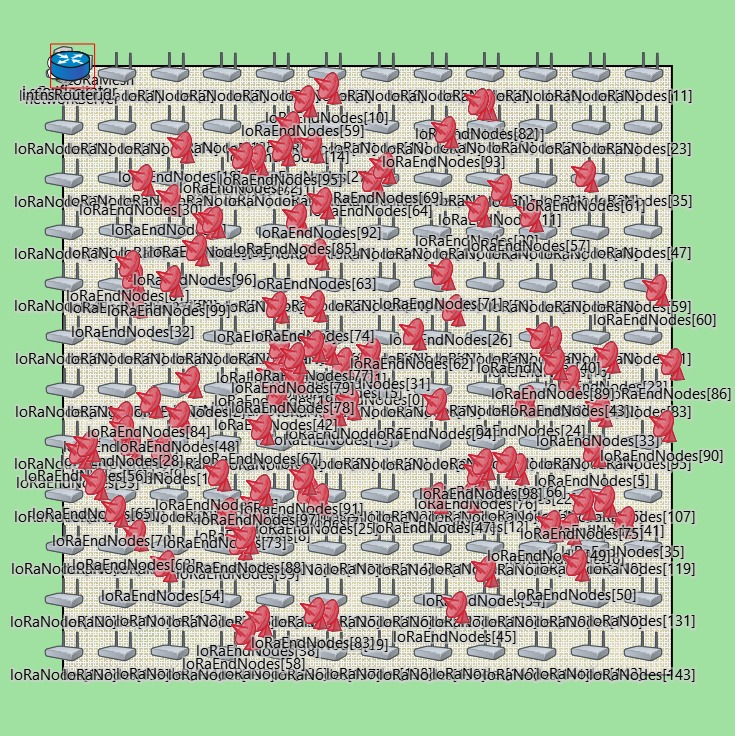
\includegraphics[width=0.5\columnwidth]{images/Nodes.jpg}
                \caption{End nodes and relay nodes}
                \label{fig:enter-label}
            \end{figure}

\newpage
\subsection{Architecture of the Simulator}
\label{sec:Architecture of the Simulator}

As explained earlier, FloRa is not a simulation tool. Omnet++ is the simulation tool and FloRa is a project done in Omnet++ with the use of inet framework. FloRa consists of protocols specifically for design a LoRaWAN. There are files for LoRa physical layer, mac layer, application layer protocols and for every and each element in the network. As and example consider a LoRa node, the node is consists of a loRaNodeapp element and a LoRaNic element. The LoRaNic consist of LoRa Radio and the LoRa Mac. The LoRa radio consists of an antena transmitter and a reciever. For each element certain types of protocols are coded in a dedicated file.Indeed, within the FloRa project framework implemented in OMNeT++, a hierarchical structure is established to systematically define and manage the various components of the LoRa network. At the core of this structure lies OMNeT++, serving as the simulation tool, while FloRa represents the project developed within this environment. Leveraging the capabilities of the INET framework, FloRa is equipped with protocols tailored specifically for LoRaWAN communication.\\

Within the FloRa project, meticulous attention is given to organizing and defining the functionalities of different layers of the LoRa network. This includes the physical layer responsible for signal transmission, the MAC layer managing medium access, and the application layer handling higher-level data processing. Each layer is delineated by dedicated protocol files, ensuring clear specification and efficient management of their respective functionalities.\\

Taking a closer look at the components of a LoRa node, such as the LoRaNodeApp and LoRANic, reveals a further level of granularity in the hierarchy. The LoRANic element encompasses essential components like the LoRa Radio and LoRa MAC, which collectively manage the radio communication aspects of the node. The LoRa Radio, in particular, includes crucial elements such as antenna transmitters and receivers, which play pivotal roles in transmitting and receiving signals within the network.\\

By establishing this hierarchical structure and meticulously defining the functionalities of each component through dedicated protocol files, FloRa enables comprehensive modeling and simulation of LoRa networks within the OMNeT++ environment. This structured approach facilitates efficient development, analysis, and optimization of LoRa-based communication systems, contributing to advancements in wireless networking technologies.\\

In the project highlighted during our literature review, the extension of incorporating a down-link feature into the FloRa framework had been successfully implemented. This enhancement facilitates direct communication between LoRa nodes, eliminating the necessity for gateways, thereby deviating from the conventional LoRaWAN architecture. Additionally, the discovered project had already implemented a routing mechanism capable of forwarding packets to known destinations. However, for our customized mesh network proposed in this project, a few additional modifications to the forwarding mechanism were necessary. Notably, traditional routing was deemed unnecessary for our specific requirements\\

            \begin{figure}[htp!]
                \centering
                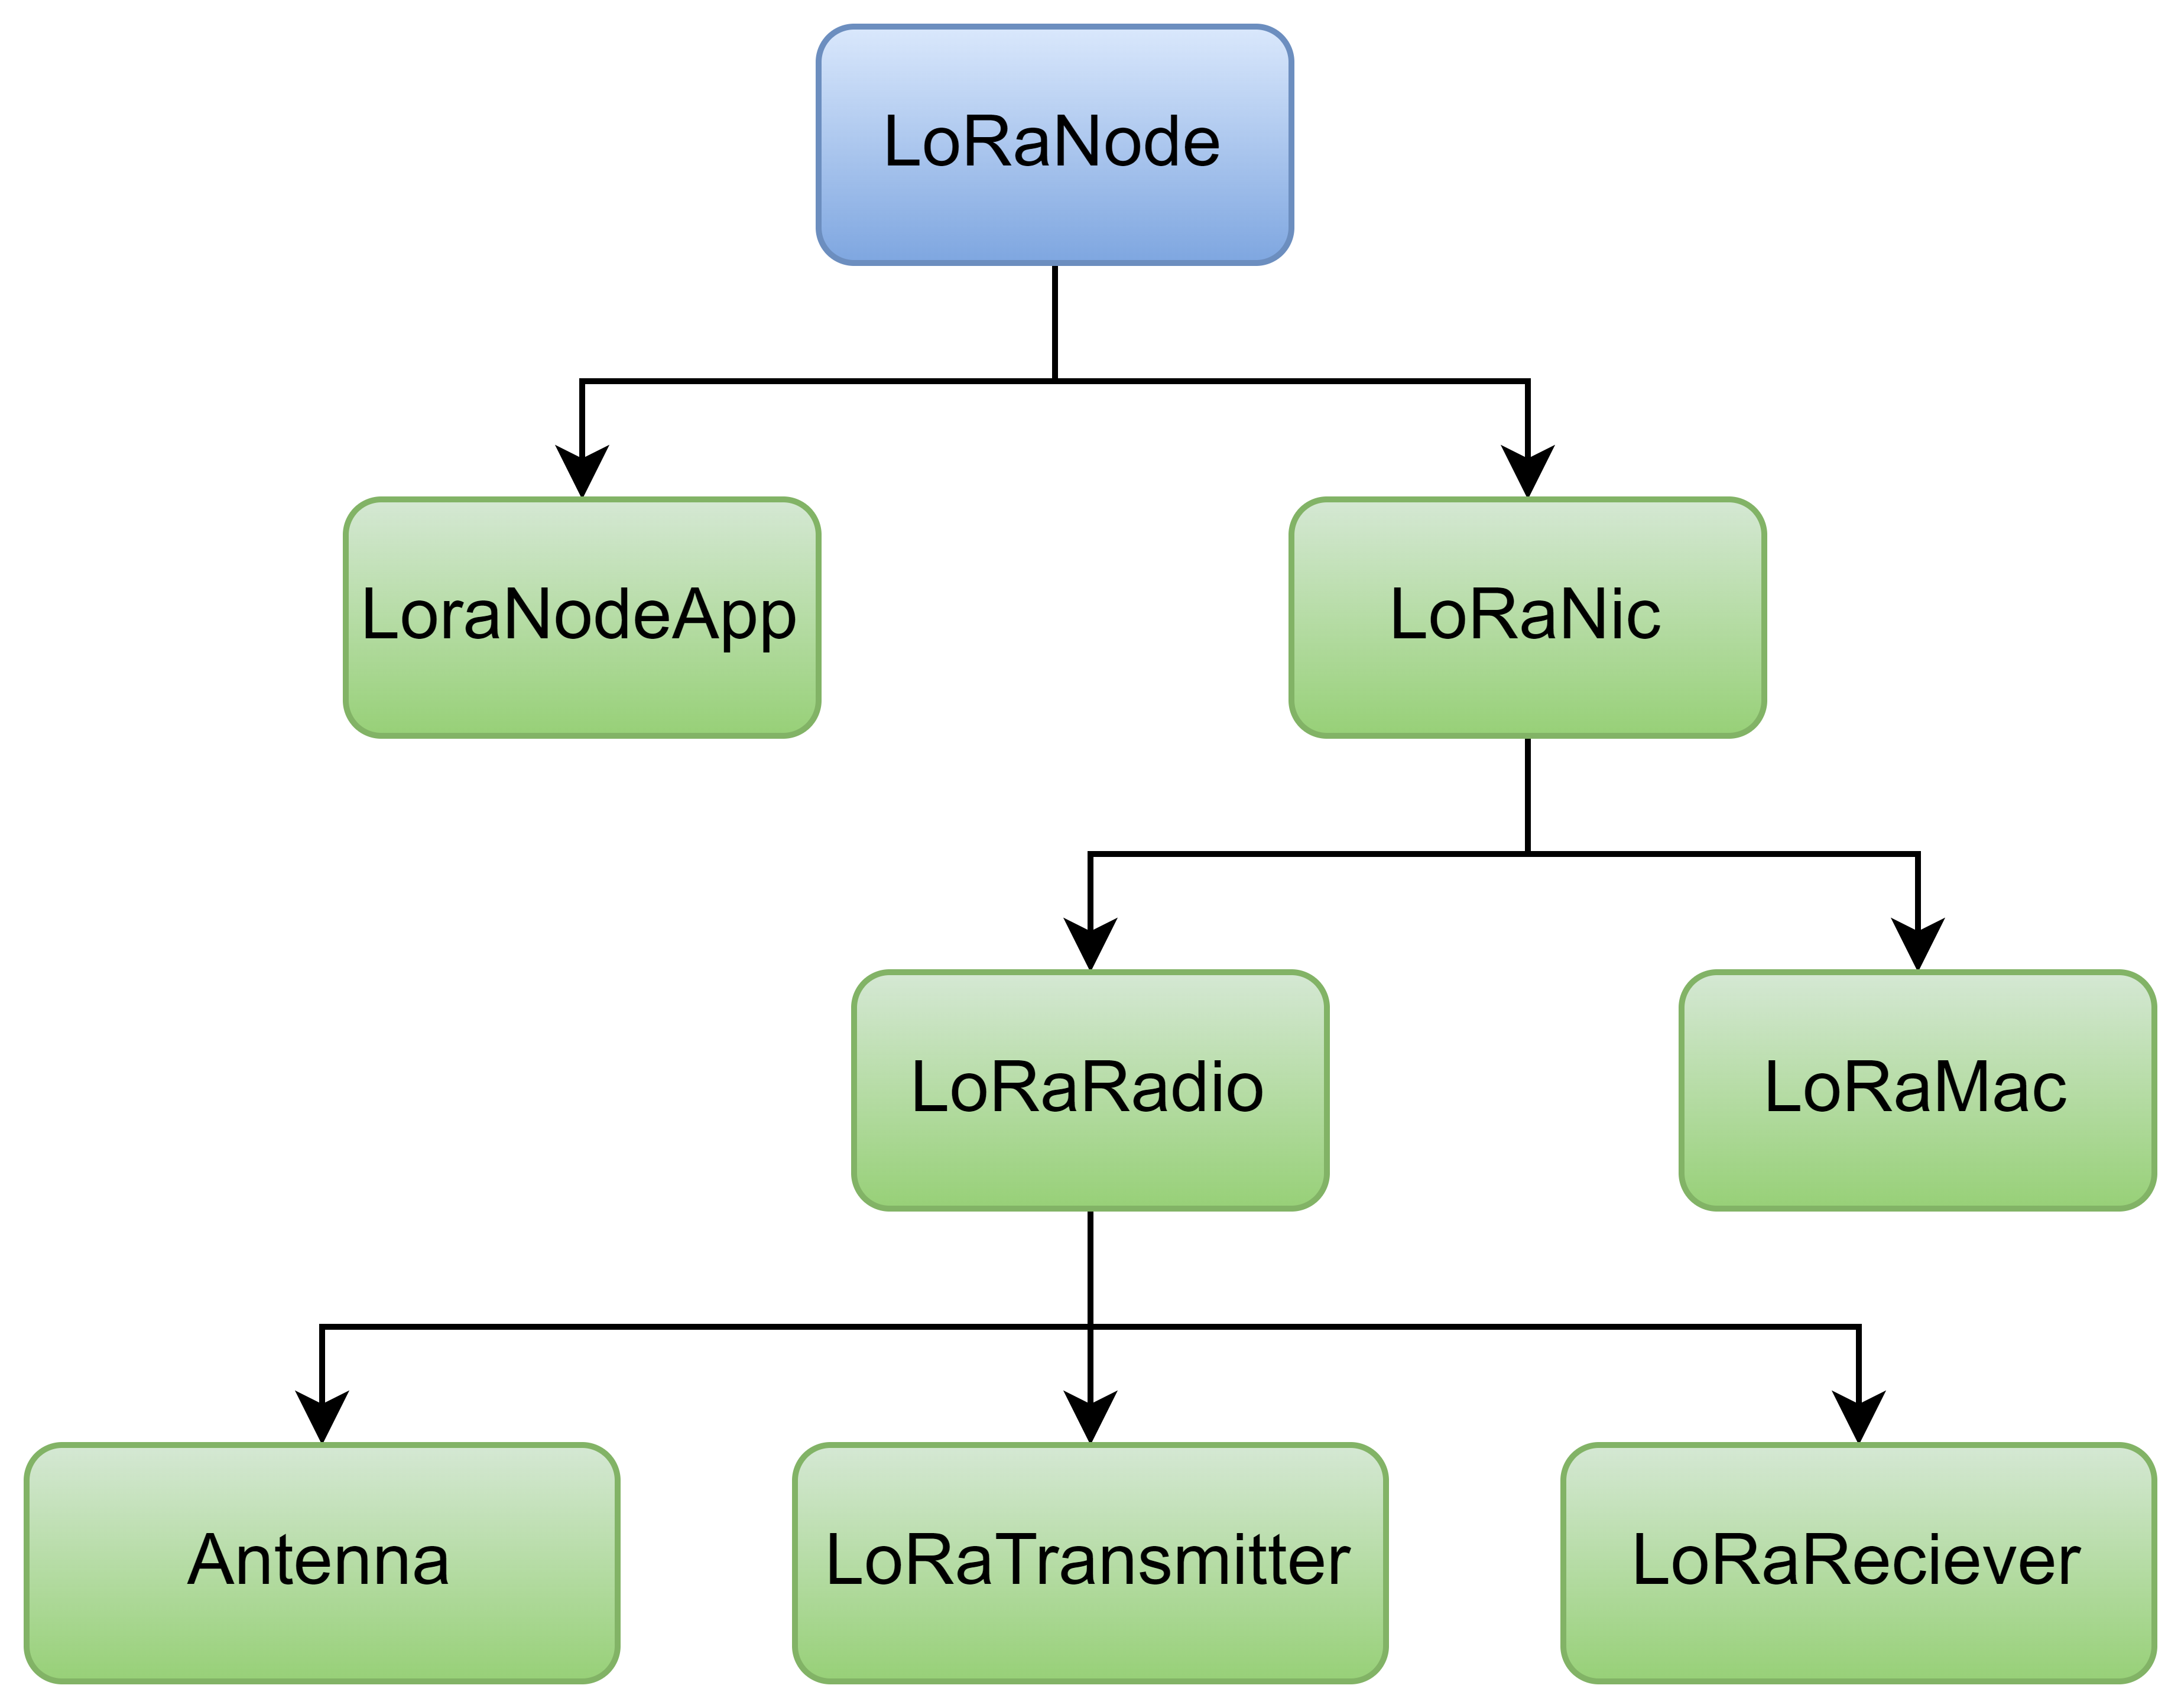
\includegraphics[width=0.7\columnwidth]{images/a.drawio.jpg}
                \caption{LoRa-Node architecture}
                \label{fig:enter-label}
            \end{figure}
            
            \begin{figure}[h!]
            \centering
                \begin{subfigure}[b]{0,4\textwidth}
                \centering
            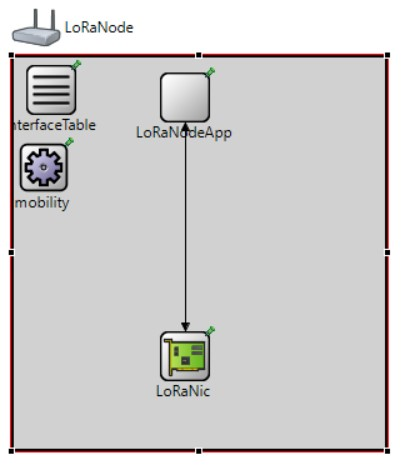
\includegraphics[width=0.8\columnwidth]{images/node.jpg}
            \caption{LoRa-Node}
            \label{fig:loRa-node}
            \end{subfigure}
            \hfill
            \begin{subfigure}[b]{0,4\textwidth}
            \centering
            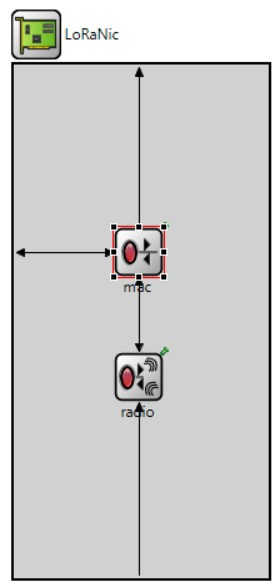
\includegraphics[width=0.5\columnwidth]{images/nic.jpg}
            \caption{LoRa-Nic}
            \label{fig:lora-nic}
            \end{subfigure}
            \hfill
            \begin{subfigure}[b]{0,4\textwidth}
            \centering
            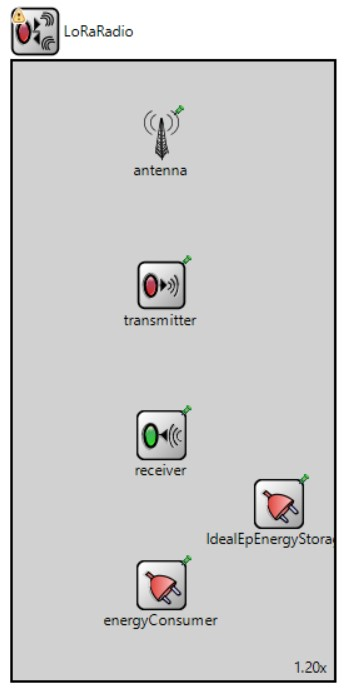
\includegraphics[width=0.6\columnwidth]{images/radio.jpg}
            \caption{LoRa-Radio}
            \label{fig:lora-radio}
            \end{subfigure}
     
            \caption{Architecture of LoRa Node}
            \label{fig:Architecture of LoRa Node}
        
\end{figure}
\newpage
After thoroughly reviewing all project files, several key files were identified for extension purposes. Within each of these files, relevant parameters and functions were examined to determine their role in the project's functionality. The following sections explain and illustrate the important files along with their respective parameters. This analysis serves as a foundational step in understanding the project structure and planning for necessary extensions and modifications.\\

\subsubsection{Package.ned file}

This file delineates the logical architecture of a .ini file, which serves as a simulation configuration file. Specifically, the package.ned file facilitates the creation of networks within the simulation environment. Within each network, parameters such as the number and type of elements, their respective icons, and the connections between different elements can be defined. Multiple networks can be specified within the package file, each representing a distinct configuration. By utilizing the executable .ini file, users can select a specific network and configure its parameters as defined within the package.ned file. This modular approach allows for flexible and customized simulation setups tailored to specific experimental requirements.\\

            \begin{figure}[h!]
                \centering
                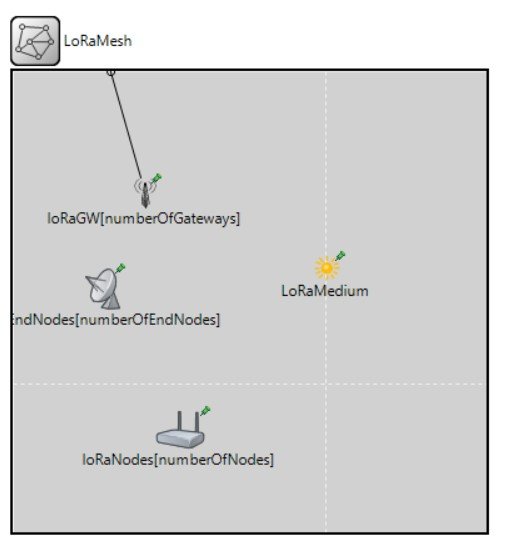
\includegraphics[width=0.5\columnwidth]{images/package.jpg}
                \caption{package.ned file}
                \label{fig:package.ned}
            \end{figure}

\subsubsection{.ini file}

The .ini file serves as the executable simulation file within FloRa, containing configurations for the network and all associated parameters. Additionally, this file includes input parameters necessary for the simulation. Furthermore, sub-configurations can be created within the main configuration, allowing for variations in parameter values. The controllable parameters encompass node parameters, node application layer parameters, propagation model parameters, energy consumer parameters, and range parameters. Upon running the configured .ini file using the simulator, results are generated, providing valuable insights into the simulated network's behavior and performance.\\

\subsubsection{LoRa-Log-Normal-shadowing files}
The Log-Normal-shadowing files are part of the LoRaPhy folder, housing protocols pertinent to the LoRa physical layer. Alongside these files, there are several others dedicated to LoRa Modulation protocols and various propagation models. For this project, the Log-Normal shadowing propagation model takes precedence. This model relies on four primary parameters: a reference distance, path-loss at the reference distance, path-loss exponent, and the standard deviation of shadowing. The tuning of these parameters is detailed in subsequent sections. Notably, these values can be configured within the .ini file, affording flexibility in customizing the simulation environment to meet specific requirements.\\

\subsubsection{LoRa Radio}
The LoRa Radio component comprises three main elements: the receiver, transmitter, and antenna. The receiver component is responsible for evaluating the conditions upon receiving a packet to determine whether it should be accepted or ignored. On the other hand, the transmitter component configures the transmission power and other LoRa parameters, such as carrier frequency, payload size, and bandwidth. Together, these components ensure effective communication within the LoRa network by managing the reception and transmission of data packets while adhering to specified parameters.\\ 
When considering the receiver, it undergoes three primary stages: initialization, packet acceptance or rejection, and completion. In the initialization stage, variables within the file are typically initialized to zero. These variables include the number of packets received, collisions encountered, received signal strength indicator (RSSI), signal-to-noise ratio (SNR), time on air, and the number of packets received below the sensitivity threshold. This stage sets the groundwork for subsequent operations, ensuring that the receiver is prepared to process incoming packets effectively.\\

In the packet reception processing stage, several functions are employed to determine the eligibility of an incoming packet for reception by the receiver. Initially, the receiver identifies whether it functions as a gateway; however, since gateways are not utilized in this project, this aspect is not elaborated upon. For receivers operating as nodes, the capability to dynamically adapt to multiple spreading factors is unnecessary, as single-channel LoRa nodes are employed. Consequently, communication within the network occurs using a single spreading factor across the entire network. Upon confirming that the receiver functions as a node, it proceeds to verify key parameters of the incoming packet, the spreading factor, bandwidth, carrier frequency, and code rate. The values of the incoming packet compared with the parameters of the receiving node. In this application all the nodes are configured for same parameters mentioned earlier.\\
Following the parameter verification, the receiver proceeds to check for potential collisions, which may occur when two or more packets are received within a defined time period. Collisions typically arise due to packets sharing the same carrier frequency and spreading factor, compounded by the capture effect. The capture effect occurs when the difference in RSSI values between two signals is less than a predefined threshold value, which, in this project, is set at 5dB with the data from the devices used. If a collision is detected, the collision counter increments, and the packets are ignored.\\

In the absence of collisions, the receiver evaluates whether the received signal strength indicator (RSSI) surpasses the sensitivity threshold corresponding to the configured spreading factor and bandwidth. This sensitivity threshold is established based on the data of the devices provided for the project. This process remains consistent across both end nodes and intermediate relay nodes, ensuring uniform handling of packet reception throughout the network.\\

Below block diagram is related to the above explained functionality of the receiver.\\
            \begin{figure}[h!]
                \centering
                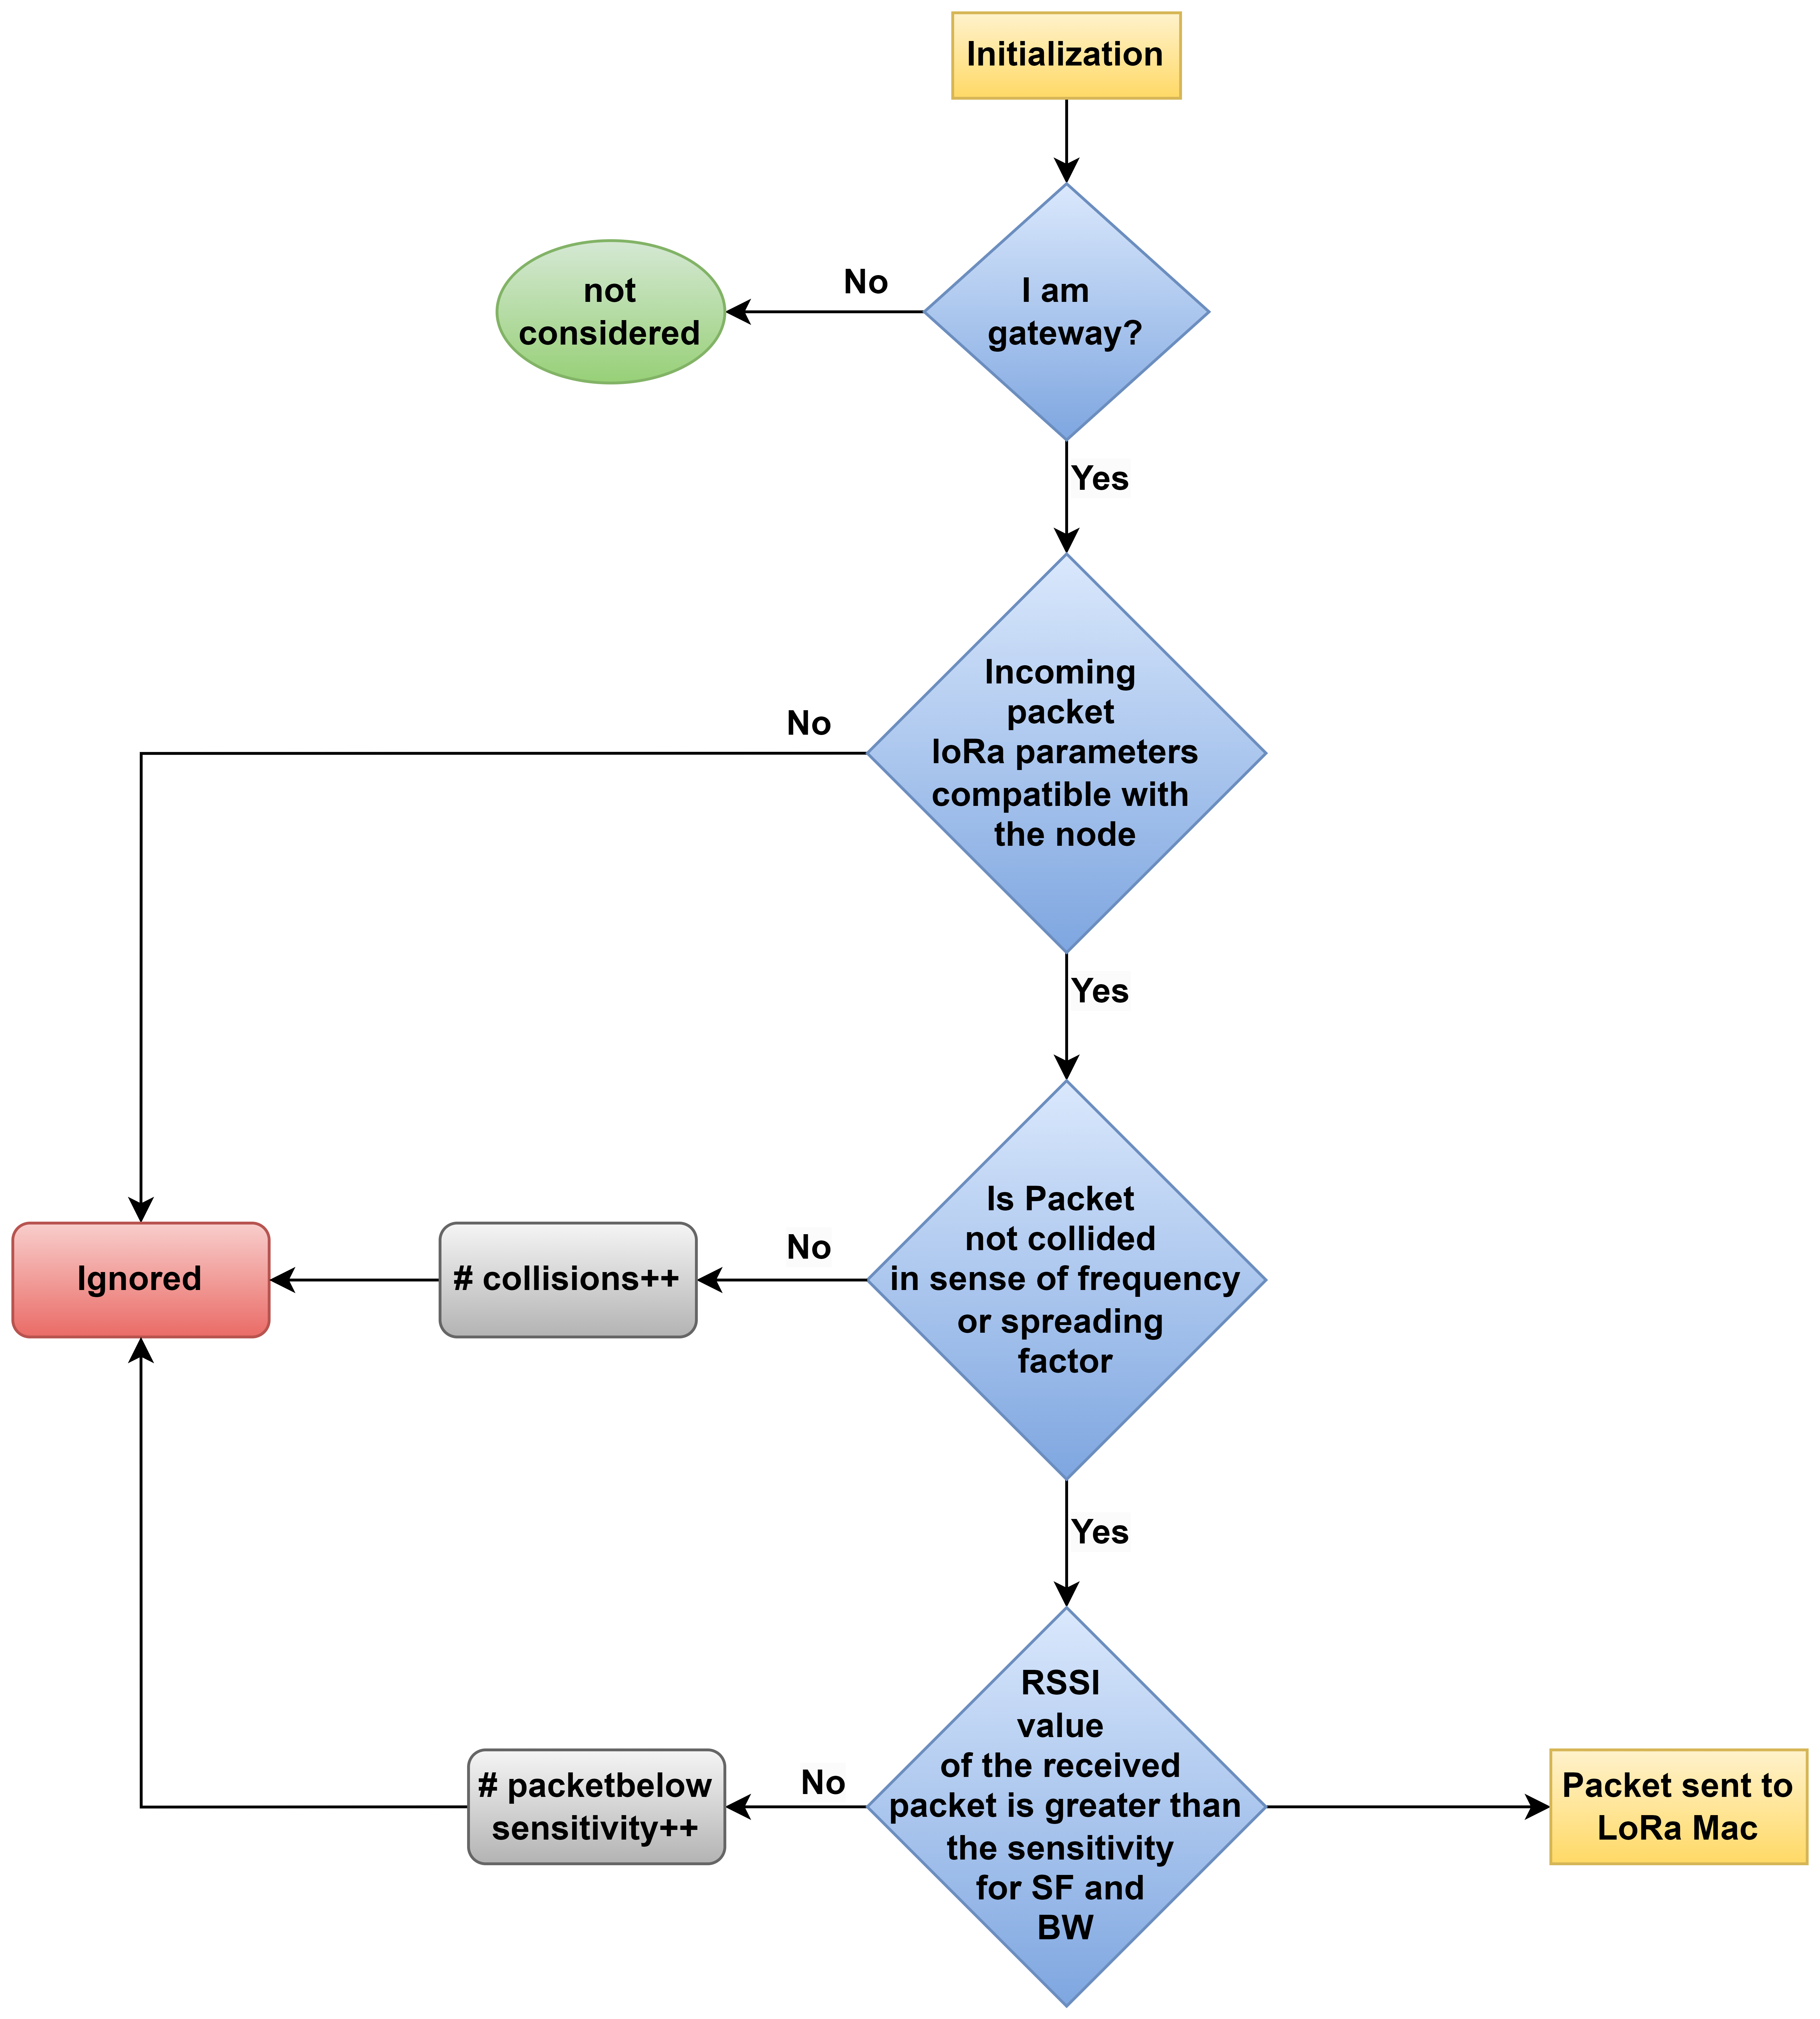
\includegraphics[width=0.8\columnwidth]{images/Parameters.jpg}
                \caption{Receiver Logic block diagram}
                \label{fig:receiver}
            \end{figure}
\newline

The transmitter component of the LoRa Radio module utilizes libraries from the inet framework to facilitate message transmission. Primarily, the transmitter extracts parameter values such as spreading factor, bandwidth, carrier frequency, code rate, and transmission power from the .ini file configuration assigned to a specific node. These parameter values are then incorporated into the transmitting packet, along with a sequence number for identification purposes. Furthermore, the antenna functionality is implemented using the IAntenna library provided by inet. This library enables the transmitter to interface seamlessly with the antenna, facilitating the transmission of packets across the network.

\subsubsection{LoRa-Node-App}
The LoRa-Node-App serves as a critical component within the simulator, playing a central role in both packet creation and the forwarding mechanism for incoming packets. This module is responsible for orchestrating the generation of packets within the network and overseeing the process by which incoming packets are forwarded to their respective destinations.\\

In the initialization phase mainly the network is created with the configuration given by the user through the .ini file. There are several number of parameters but the most important parameters are explained below.\\\\
\textbf{routing metric}\\\\
Initially, the simulator tool identified through the literature review, as mentioned earlier, employed a routing protocol to facilitate packet forwarding to designated destinations. Within this framework, seven distinct routing metrics were defined. In our project, we extended this functionality by utilizing the routing metric parameter to differentiate between LoRa end nodes and LoRa relay nodes. Specifically, the routing metric is assigned a value of 0 for end nodes and 1 for relay nodes. During the initialization phase, this routing metric value for each node within the simulation network is considered, allowing for the establishment of the requisite number of end nodes and relay nodes. Additionally, distinct icons are assigned to end nodes and relay nodes during the initialization phase to visually differentiate between them.\\\\
\textbf{deployment type}\\\\
After assigning routing metrics to differentiate between end nodes and relay nodes, each node is allocated a unique node ID. Subsequently, nodes are positioned within the network according to predefined deployment types, which include grid, circle, edge, and specific location placements. For relay nodes, a grid-based deployment strategy is employed, with slight random variations introduced to each node's position. The grid separation is carefully determined based on factors such as spreading factor and propagation model parameters, tailored to the specific environmental conditions. End nodes, on the other hand, are placed in a circular configuration with a radius of 30km. Initially, the primary end node, designated as end-node-0, is positioned at the network's center, as it initiates the packet transmission process. This initial message, known as a self-packet, in the network for the certain node. The eligibility to sent a self-packet from only the end-node-0 is also set by a boolean parameter known as "onlyNode0SendsPackets".\\\\
\textbf{packetTTL}\\\\
This parameter, known as the packet time-to-live (TTL), essentially determines the maximum number of hops a packet is permitted to traverse within the network. With each hop, the packetTTL value is decremented by 1. In this context, the packetTTL value is configured to align with the number of relay nodes present in the network, as each relay node represents a hop that must be traversed to reach its destination. Additionally, the packetTTL value can serve as a mechanism to control the forwarding process within the network.\\\\
\textbf{Other parameters}\\\\
There are other parameters to generate results, keep the track of sent, forwarded, routed, deleted messages. And also, there are parameters taken for LoRa Modulation. All the values are used in generation of elog files, scaler and vector files at the end of the simulation of a certain network.\\

In the below section the main functionality of forwarding and generating packet explained. In this project all the relay nodes have the capability to forward packets. But the same packet is not forwarded twice.\\\\
\textbf{Packet generation and forwarding mechanism}\\\\
In the absence of routing protocols in this application, request and acknowledgement packets are not utilized within the network. Consequently, only data packets are propagated throughout the entire network. As a result, functionalities pertaining to the handling of other types of messages, such as request and acknowledgement packets, have been eliminated from the system. This streamlined approach simplifies the network architecture and focuses exclusively on the transmission and reception of data packets, optimizing efficiency and resource utilization within the network.\\
A transmiting self packet has the source node-ID and the LoRa parameters with it. In each relay node if forwarding occurs the relay node ID is also added to the packet. In each relay node, it is checked whether the incoming packet is forwarded once using the ID's in the packet and also in the end nodes it check whether the self-packet come back to the generated node. Below block diagram gives a breif understanding of the forwarding mechanism.\\
\newpage
            \begin{figure}[h!]
                \centering
                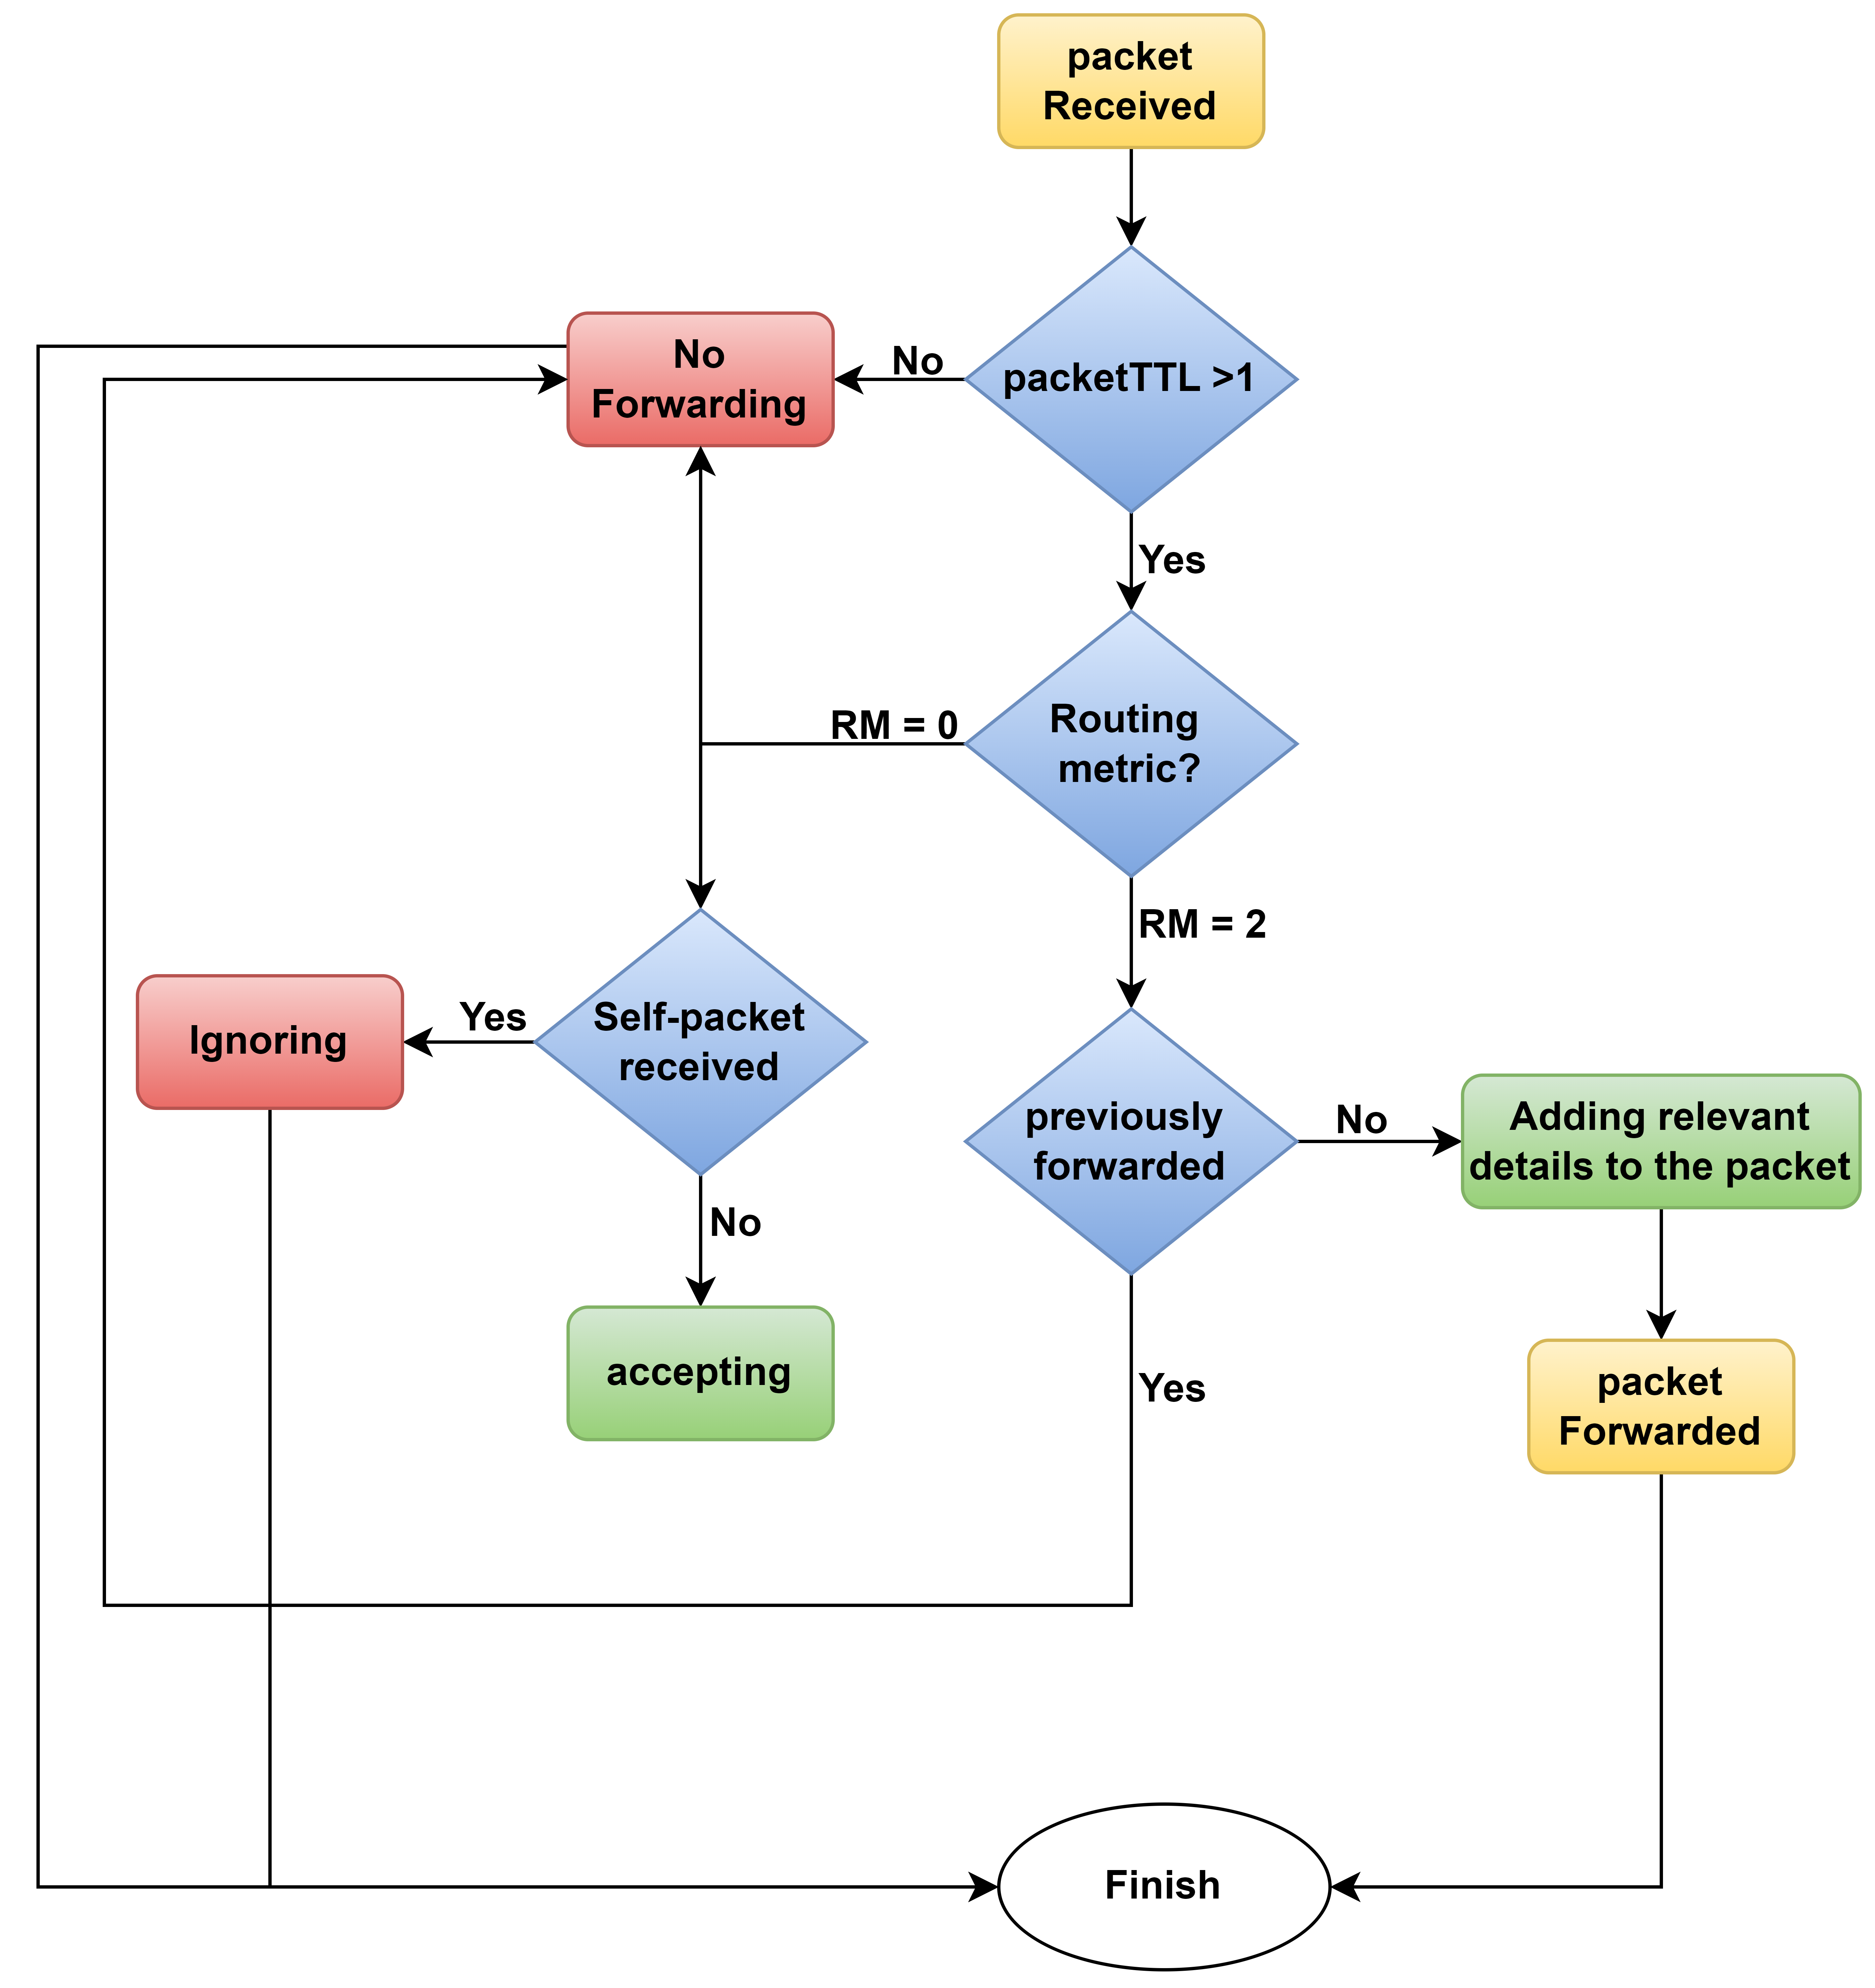
\includegraphics[width=0.9\columnwidth]{images/forwarding mechanism.jpg}
                \caption{forwarding mechanism}
                \label{fig:forwarding mechanism}
            \end{figure}
Below figure shows the basic propagation path of a packet from one node to another node. The receiving node can be a relay node or an end node.
\newpage
            \begin{figure}[h!]
                \centering
                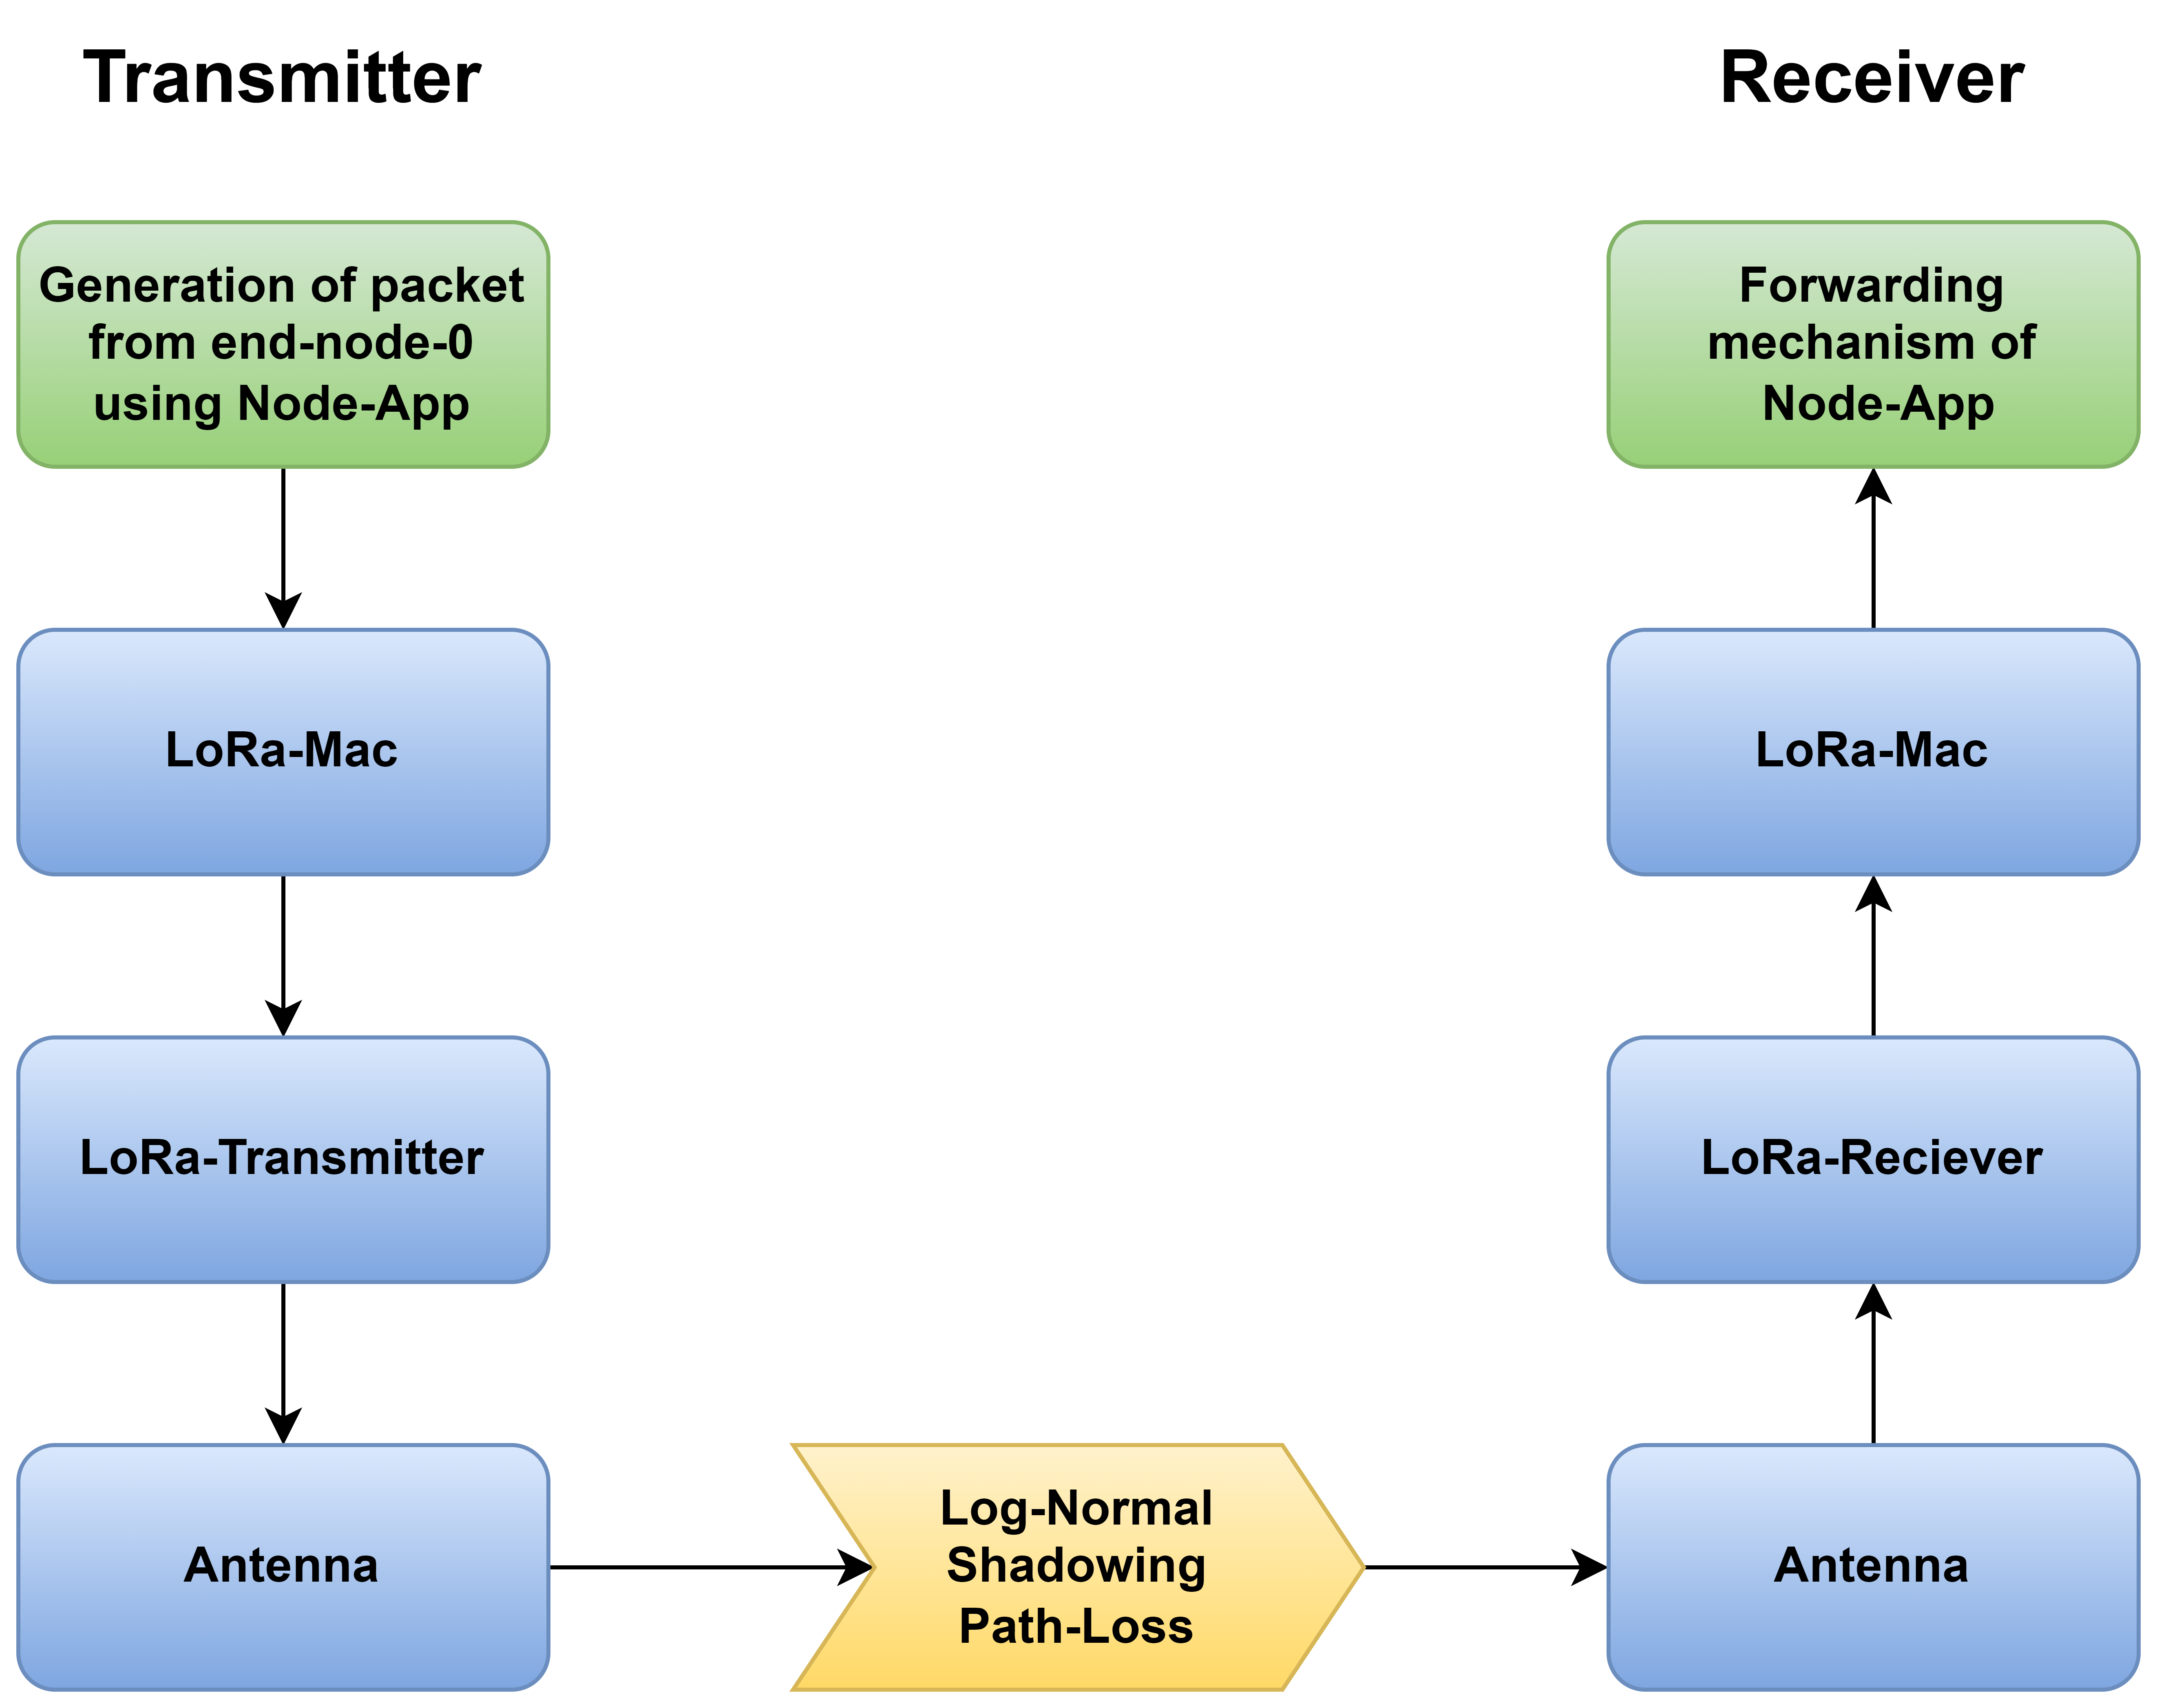
\includegraphics[width=0.7\columnwidth]{images/packet propagation path.jpg}
                \caption{packet propagation path}
                \label{fig:packet propagation path}
            \end{figure}


 



%------------------------------------------------------------------------------------------

\section{Propagation Model}
\label{ch:Propagation_model}

\subsection{Importance of the Propagation Model}
\label{sec:Propagation Model}
The success of our project depends heavily on how well we manage the way signals travel. Although LoRa technology is great for long-distance communication without using too much power, it can still be affected by things like the environment and obstacles in the way. That's why it's really important for us to predict how far the signals can reach accurately using a tuned propagation model. In our plan, we're using two types of nodes: end-nodes and relay nodes. End nodes are placed near users and the messages are generated here. Relay nodes help spread messages throughout the network. The objective is to cover up to 30km radius area at a minimum time.
As explained earlier in this report, factors such as spreading factor, bandwidth, code-rate, and transmission power are crucial parameters in LoRa communication. Increasing the spreading factor not only extends the total time required to transmit a packet but also enhances the transmission distance. Hence, it becomes essential to identify the optimal point where we can transmit data over a specific distance in the shortest time possible. The proposed architecture introduces a multi-hop transmission approach to address this challenge. This approach involves breaking down longer distances, requiring higher spreading factors, into multiple shorter hops utilizing lower spreading factors. By doing so, we can cover greater distances within significantly reduced time frames. Selection of a suitable spreading factor and nodes density is dependent on the environment. Therefore, to simulate the environment effect propagation model is a must.

\subsection{Log-Normal Shadowing Model}
\label{sec:Log-Normal}
The Nodes are placed in a hilly and a windy environment. In hilly and windy environments, LoRa communication encounters unique challenges due to the irregular terrain and fluctuating environmental conditions. Traditional propagation models often fail to adequately capture the complexities of signal propagation in such dynamic landscapes. Log-Normal shadowing, however, offers a more sophisticated approach by incorporating statistical variations in signal strength, making it particularly well-suited for these environments.\\\\
In hilly terrain, the elevation changes can obstruct direct line-of-sight communication paths, resulting in signal attenuation and shadowing effects. Log-Normal shadowing effectively models these variations by incorporating random fluctuations in signal strength caused by terrain irregularities. In windy conditions can exacerbate signal attenuation by causing foliage and other obstacles to sway, altering the propagation environment dynamically. Log-Normal shadowing provides resilience to such fluctuations by offering a statistical framework to account for these environmental changes over time. Therefore,  Log-Normal shadowing facilitates precise estimation of communication range by considering both deterministic path loss and stochastic shadowing effects. This allows network planners to design robust communication links that account for terrain variations and environmental dynamics, leading to more efficient network coverage and improved performance.

The Log-Normal Propagation model is as follows.\\
\begin{equation}
PL(d) = PL(d_0) + 10 \cdot \alpha \cdot \log_{10}\left(\frac{d}{d_0}\right) + \text{Normal}(0, \sigma)
\end{equation}
\begin{itemize}
    \item $\text{PL}(d)$ is the path loss at distance $d$.
    \item $\text{PL}(d_0)$ is the reference path loss at a reference distance $d_0$.
    \item $\alpha$ is the path loss exponent.
    \item $\text{Normal}(0, \sigma)$ represents the log-normally distributed shadowing effect with mean 0 and standard deviation $\sigma$.\\
\end{itemize}
The reference path loss term has to be the free space path loss in a known distance. Therefore, a practical test was done in the university playground, University of Moratuwa to found out the actual value of the term using Lilygo devices. The known distance was approximately 190m and the observed path loss was 96dB. There was line of sight between the 2 nodes.

            \begin{figure}[h!]
            \centering
            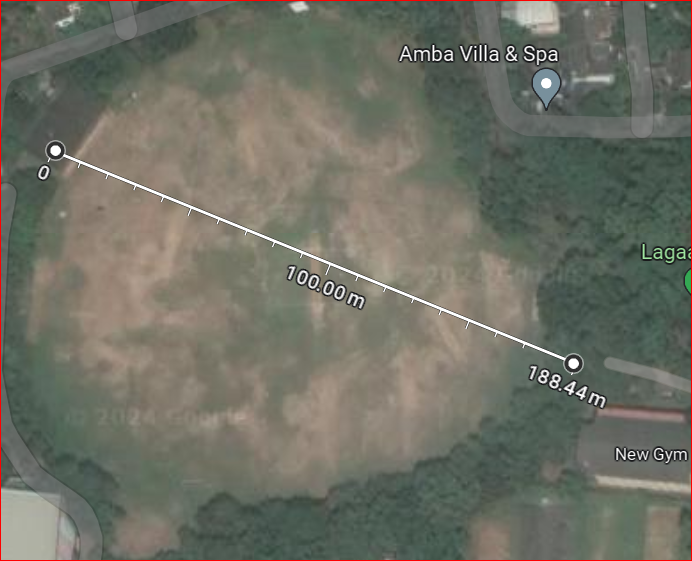
\includegraphics[width=0.7\columnwidth]{images/ground.jpg}
            \end{figure}
The next term is related to the deterministic path loss. The parameter path loss exponent($\alpha$), depends on the environment. The path loss term is the rate of decrease of the signal power with the increase of the distance. It characterizes the attenuation of the signal as it propagates through the medium and interacts with the environment. This parameter is one of the most important parameters in the model which has to be determined prior. The value of the parameter determines the signal coverage, node density, and link budget. The table given below is a reference for the path loss exponent values in different environments. Further details can be refer through [6]\\
\begin{center}
    
\begin{tabularx}{0.8\textwidth} { 
  | >{\raggedright\arraybackslash}X 
  | >{\centering\arraybackslash}X 
  | >{\raggedleft\arraybackslash}X | }
 \hline
 \textbf{Environment} & \textbf{Path-loss Exponent Value}  \\
 \hline
 Free Space  & 2  \\
\hline
 Urban Area Cellular Radio & 2.7 to 3.5  \\
 \hline
 Shadowed  Urban Cellular Radio  & 3 to 5  \\
 \hline
  Inside a Building line of sight & 1.6 to 1.8  \\
 \hline
 Obstructed in building  & 4 to 6  \\
 \hline
 Obstructed in factory  & 2 to 3  \\
  \hline
\end{tabularx}
\end{center}

The next term is related to the stochastic shadowing effect which is log-normally distributed with 0 mean and standard deviation of $\sigma$. The $\sigma$ value is dependent with the environment, for highly shadowed area the $\sigma$ value increases. This is the other most important term in the propagation model to determine the coverage area, and node density. \\

\subsection{Fine tuning parameters}
\label{sec:parameters}

For each environment path-loss exponent value and the standard deviation value has to be tuned properly to simulate and predict the coverage range and node density. The values may differ for each cases.
 
Even though reference values are given to certain environments, better approach is to find-out the value for path-loss exponent and the standard deviation using field experiments combined with simulations and theoretical findings .Field measurement can be taken as follow. Conduct field measurements by deploying transmitters and receivers at various distances in the target environment. Measure the received signal strength at each distance, taking into account factors such as terrain, obstacles, and environmental conditions. Plot the received signal power against distance on a logarithmic scale (dB vs. log-distance) to observe the path loss behavior.\\

Throughout this project several experiments were done in different types of environments such as, urban low shadowed, urban highly shadowed and university environment. Using the data collected, observing and analysing the parameters and fine tuning is done using the simulation tool.

\subsubsection{Theoretical Variation of path-loss}
The following details are related to the theoretical variation of the path-loss with distance, path-loss exponent and the standard deviation $\sigma$.\\

The variations are related to 17dBm transmission power with a 2dBm receiver antenna gain. The spreading factor determines the duration of each symbol, affecting the time and energy required for transmission. In your case, spreading factors 7, 8, and 9 are specifically considered due to their relevance to the proposed network architecture. The reason for selecting these spreading factors is based on the architecture's strategy of transmitting messages over long distances using multiple hops of lower spreading factor values instead of using a higher spreading factor to minimize transmission latency. This approach is designed to optimize the trade-off between transmission range and latency, considering the specific requirements and constraints of the network. By utilizing spreading factors 7, 8, and 9, the network aims to achieve efficient communication over extended distances while minimizing the time required for transmission. This strategy enables the network to cover large geographic areas effectively while maintaining acceptable latency levels, enhancing the overall performance and reliability of the system.\\

To initially analyze the path loss behavior without considering random shadowing, the first step is to plot the path loss against distance, and path loss exponent $\alpha$, for different spreading factors while assuming no shadowing ($\sigma$). The following graphs illustrate this variation for spreading factors 7, 8, and 9, with a fixed transmission power of 17 dBm. This power level represents the maximum allowable transmission power for the devices used in this project. In each graph, a plane is drawn to represent the maximum sensitivity for each spreading factor. This plane indicates the threshold below which received signals may be reliably detected by the receiver. By comparing the actual path loss values with these sensitivity planes, we can assess the coverage range and performance of the communication system under different spreading factors.

These initial plots serve as a baseline for further analysis and optimization of the system parameters, including the path-loss exponent and standard deviation, considering the random shadowing effects. By iterative refining these parameters and conducting additional simulations or experiments, we can fine-tune the system to achieve optimal coverage range and node density in various environments.\\

The combined graph below illustrates how the distance varies with the path-loss exponent $\alpha$ for spreading factors 7, 8, and 9. By analyzing the interception points of the points of each graph and the plane representing the maximum sensitivity, we can determine the relationship between distance, path-loss exponent, and spreading factor. Only values from 3 to 5 are taken for alpha considering the reference table given above, since in the real application nodes are placed in an urban environment. For further details and clarification access this \href{https://colab.research.google.com/drive/1Qwp6aWWC2aQOnpKNQn7393luhTESWTYo#scrollTo=UuDD7vf8jCxN}{link}. \\


            \begin{figure}
     \centering
     \begin{subfigure}[b]{0,45\textwidth}
         \centering
         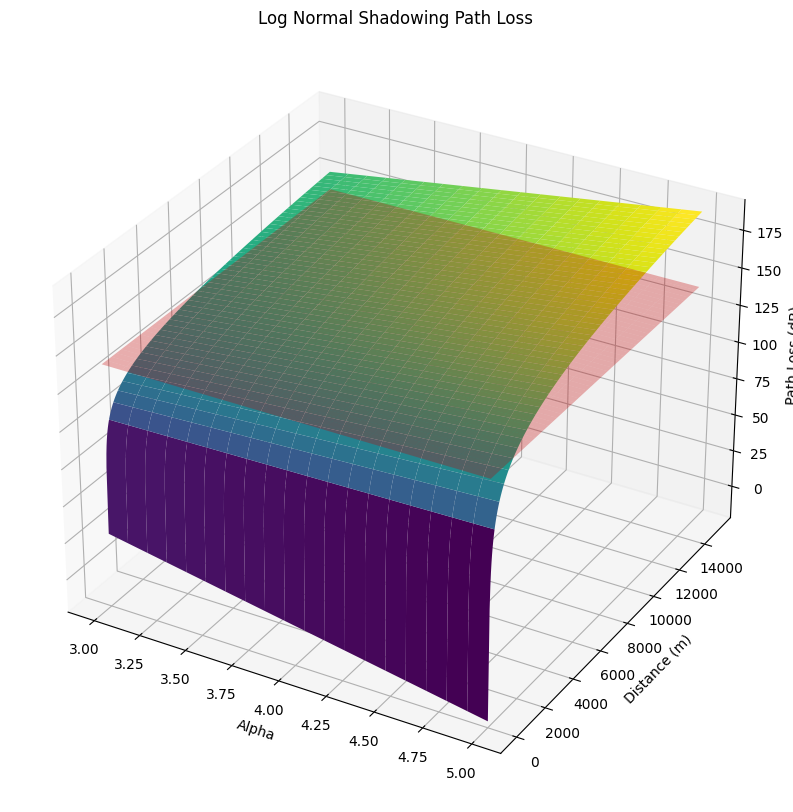
\includegraphics[width=\textwidth]{images/sf-7.jpg}
         \caption{SF-7}
         \label{fig:sf-7}
     \end{subfigure}
     \hfill
     \begin{subfigure}[b]{0,45\textwidth}
         \centering
         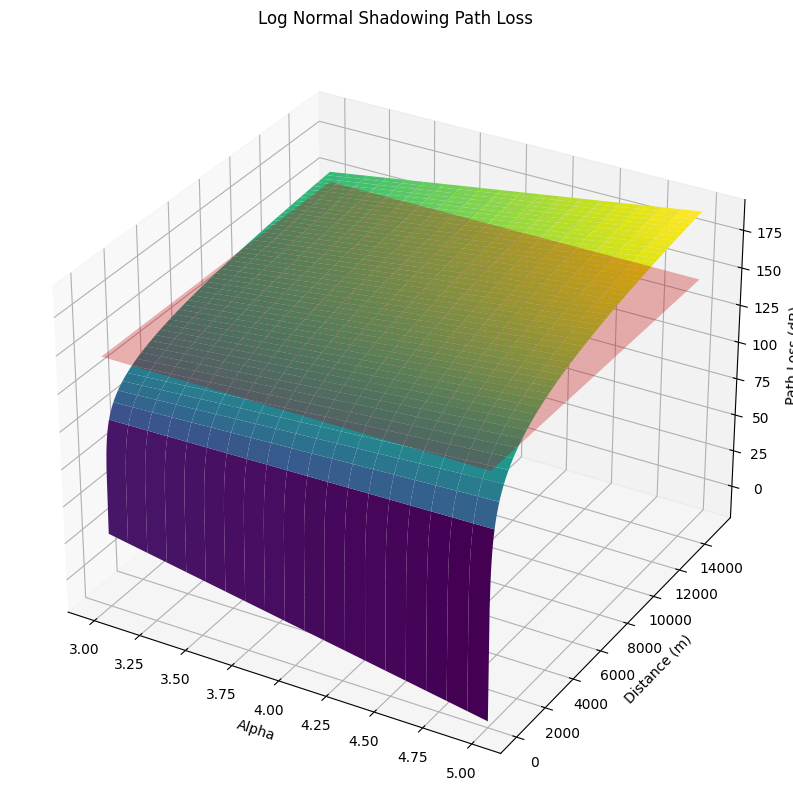
\includegraphics[width=\textwidth]{images/sf-8.jpg}
         \caption{SF-8}
         \label{fig:SF-8}
     \end{subfigure}
     \hfill
     \begin{subfigure}[b]{0,45\textwidth}
         \centering
         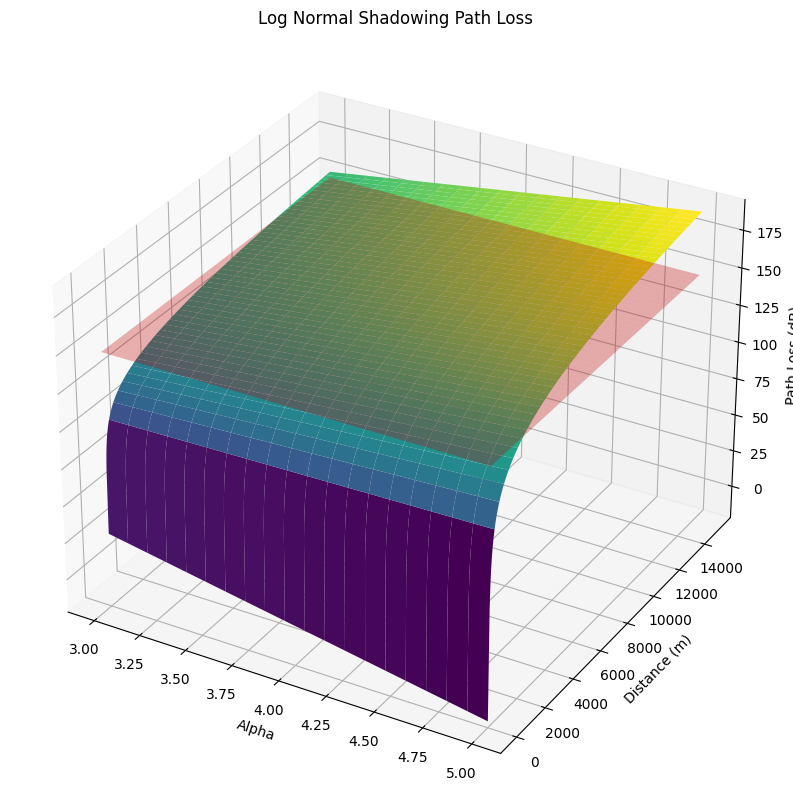
\includegraphics[width=\textwidth]{images/sf-9.jpg}
         \caption{SF-9}
         \label{fig:sf-9}
     \end{subfigure}
        \caption{Variation of path-loss with alpha and distance}
        \label{fig:initial graphs}
\end{figure}

%(\url{https://colab.research.google.com/drive/1Qwp6aWWC2aQOnpKNQn7393luhTESWTYo#scrollTo=UuDD7vf8jCxN}).\\

% \href{https://colab.research.google.com/drive/1Qwp6aWWC2aQOnpKNQn7393luhTESWTYo#scrollTo=UuDD7vf8jCxN}{Click here}

Analysis of the graph provides valuable insights into selecting the correct spreading factor value to achieve maximum distance in minimum time while considering environmental variations. It allows us to optimize the communication system by balancing the trade-off between spreading factor, transmission distance, and transmission time. By choosing an appropriate spreading factor based on the desired communication range and latency requirements, we can enhance the efficiency and reliability of the system in diverse environmental conditions.
            \begin{figure}
                \centering
                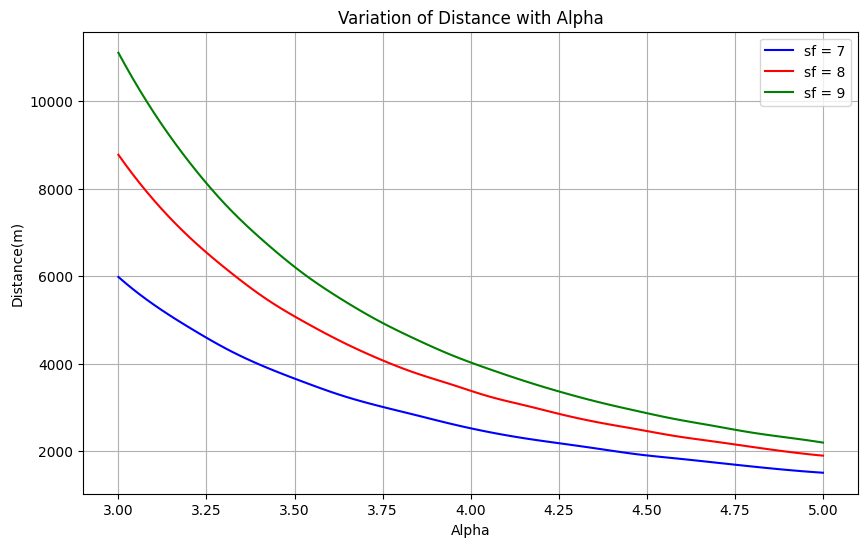
\includegraphics[width=0.7\columnwidth]{images/sigmazero.jpg}
                \caption{Distance variation with $\alpha$ for $\sigma=0$}
                \label{fig:enter-label}
            \end{figure}

The figure illustrates that the communication range between two separated nodes decreases as the spreading factor increases. However, the crucial analysis lies in examining the distance for a certain path-loss exponent ($\alpha$) value across different spreading factors. The difference in distances does not double for each increase in spreading factor. For instance, at $\alpha$=3.5, the distances for spreading factors 7, 8, and 9 are approximately 3600m, 5000m, and 6100m, respectively. Despite the increase in distance, the time to transmit a message doubles with each increment in spreading factor. For example, using spreading factor 7 takes about 60ms, spreading factor 8 takes 99ms, and spreading factor 9 takes 199ms.

This observation highlights the importance of selecting the appropriate spreading factor to balance factors such as reliability, latency, and node density. Based on the above, most of the practical experiments were done with the use of spreading factor 8.\\


The updated graphs below illustrate the variation of distance with the path-loss exponent ($\alpha$) for different standard deviation ($\sigma$) values in the stochastic variation of path-loss for certain spreading factor values. The mean minimum distance of 50 iteration for a given $\sigma$ value is plotted in the graph since the variation is completely random.\\

These enhanced visualizations provide a more comprehensive understanding of how changes in both $\alpha$ and $\sigma$ impact the communication range under stochastic path-loss conditions. By examining the interplay between $\alpha$, 
$\sigma$, and distance across various spreading factors, we can gain deeper insights into the system's behavior and optimize its parameters accordingly.

This upgraded version of the graphs facilitates a more nuanced analysis, enabling us to identify the optimal combinations of $\alpha$ and $\sigma$ for each spreading factor. By considering factors such as reliability, latency, and environmental variations, we can fine-tune the system parameters to enhance performance and ensure robust connectivity in diverse operating conditions.

 
        \begin{figure}
     \centering
     \begin{subfigure}[b]{0.45\textwidth}
         \centering
         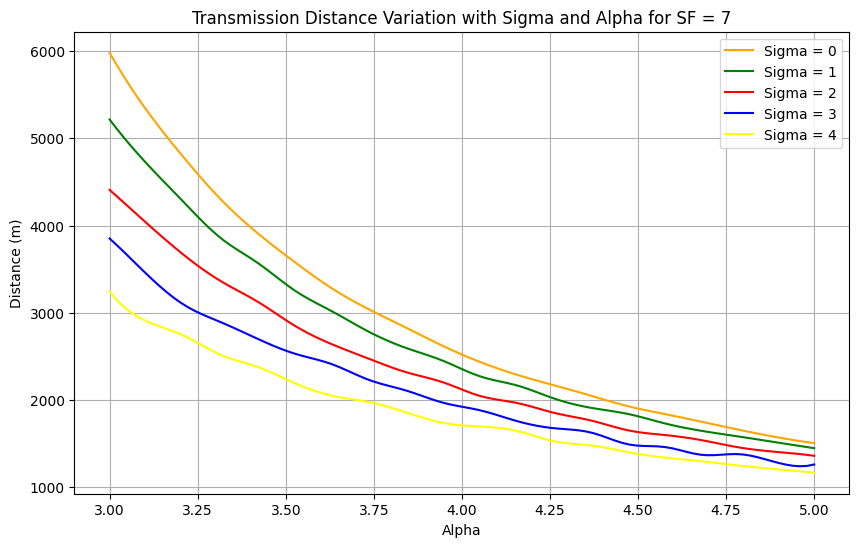
\includegraphics[width=\textwidth]{images/sigma - 7.jpg}
         \caption{SF-7}
         \label{fig:sf-7}
     \end{subfigure}
     \hfill
     \begin{subfigure}[b]{0.45\textwidth}
         \centering
         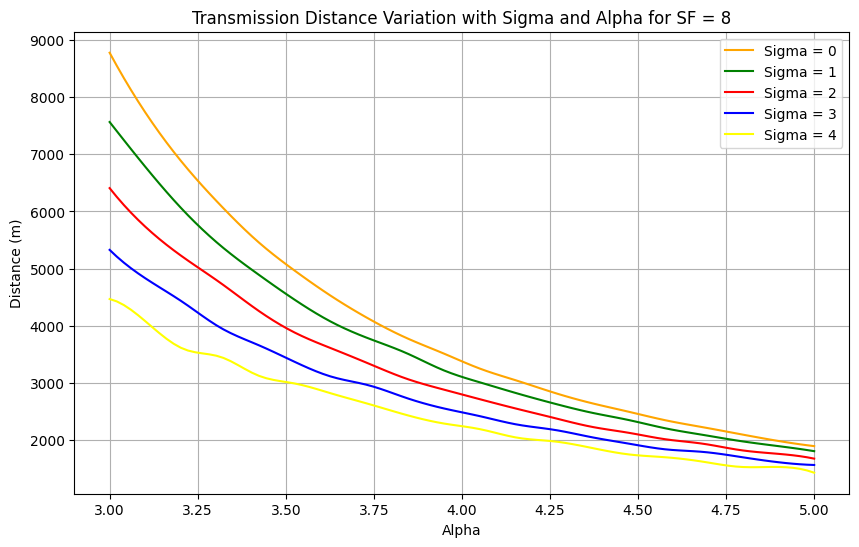
\includegraphics[width=\textwidth]{images/sigma - 8.jpg}
         \caption{SF-8}
         \label{fig:SF-8}
     \end{subfigure}
     \hfill
     \begin{subfigure}[b]{0.45\textwidth}
         \centering
         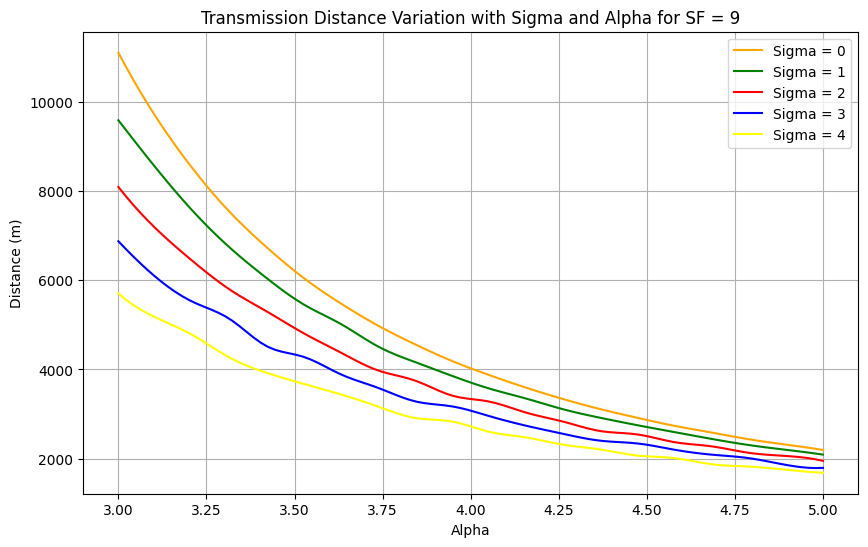
\includegraphics[width=\textwidth]{images/sigma - 9.jpg}
         \caption{SF-9}
         \label{fig:sf-9}
     \end{subfigure}
        \caption{Variation of Distance with alpha for different spreading factors and shadowing}
        \label{fig:initial graphs}
\end{figure}

Indeed, the previous explanations hold true for the updated graphs as well. Additionally, it's notable that the minimum distance required for reliable data transmission decreases as the $\sigma$ value increases.

With this information, determining the path-loss exponent($\alpha$) and the standard deviation($\sigma$) value for a given environment becomes crucial. Once these parameters are identified, and a spreading factor is predetermined for the entire communication system, the separation distance between nodes can be accurately estimated using the provided graphs. Consequently, based on the separation distance and other system parameters, such as transmission power and receiver sensitivity, the node density can be determined effectively.\\

The subsection below describes a methodology for determining the path-loss exponent($\alpha$) aand the standard deviation($\sigma$) through a combination of small-scale experiments and a simulation tool developed specifically for this project.

\subsubsection{Finding parameters using small-scale experiments and simulation tool}

To determine the combination of values for path-loss exponent($\alpha$) and standard deviation($\sigma$), a combination of small-scale practical testing in the target environment and developed simulation tool is used. In this process, nodes with a minimum transmission power of 2 dBm or higher are deployed in the environment. These nodes are placed at various distances from each other, and a certain number of data packets (at least 150) are transmitted between transmitter and receiver nodes. More transmission may give a more accurate results for the values determined.\\

Accurate measurement of the distances between nodes is crucial for obtaining reliable results. At the receiver nodes, the Received Signal Strength Indicator (RSSI) values are recorded for each transmitted data packet. These RSSI values provide insights into the signal strength received at each receiver node. By analyzing the distribution of RSSI values, the standard deviation ($\sigma$) and the mean value of the RSSI values can be calculated, representing the variation in signal strength due to factors such as path loss and environmental conditions.\\

Determining the alpha value necessitates the utilization of a developed simulation tool, calculated standard deviation, mean value, and accurate distance measurements. Initially, within the simulation tool, a transmitter and receiver are positioned at the same distance as in the practical experiment. Essential parameters including spreading factor, transmission power, and standard deviation($\sigma$) values are meticulously configured within the simulation data to mirror real-world conditions. Subsequently, a predetermined number of packets are transmitted between the transmitter and receiver in the simulation, aiming to replicate scenarios akin to the real environment. The simulated data is then analyzed to compute the mean value of the Received Signal Strength Indicator (RSSI) values for the predicted $\alpha$ value. By comparing the mean RSSI values obtained for different alpha values, the most accurate representation of the path-loss exponent($\alpha$) can be discerned. To further validate the selected alpha value, additional receiver data from different distances is employed. This involves checking observed RSSI values against those predicted based on the selected $\alpha$ and $\sigma$ values. Through this iterative process of simulation and validation, an accurate determination of both $\alpha$ and $\sigma$ values is attained, ensuring the reliability and effectiveness of the communication system in real-world scenarios.\\

After calculating the values for $\alpha$ and $\sigma$ using the small-scale experiment, the focus shifts to determining the maximum feasible separation for reliable data communication using theoretical graph data and the simulation tool. This crucial insight allows for the establishment of an optimal node density corresponding to a specific spreading factor. Importantly, the values of $\alpha$ and $\sigma$ remain constant regardless of the spreading factor, as they are solely determined by the environmental conditions. Therefore, with the $\alpha$ and $\sigma$ values in hand, network planners can easily determine the most suitable spreading factor and node density to ensure efficient and reliable communication within the network. This streamlined approach facilitates effective network optimization, enabling the deployment of resources in a manner that maximizes performance while minimizing latency and other potential constraints.

%------------------------------------------------------------------------------------------
\section{Firmware Development}\label{ch:firmware}
In the architecture we have mainly following types of devices,
\begin{itemize}
    \item End Node
    \item Relay Node(Forwarder)
    \item Custom Gateway
\end{itemize}

\subsection{Design Adaptations and Optimizations}

To address the time-sensitive nature of the mesh network, we've implemented optimizations in our firmware and architectural design, thereby maximizing device and network utilization.

\subsubsection{Radio-lib}

% ToDO mention about the Radiolib

Radiolib is a highly popular and versatile library for wireless communication experimentation in the field of electronics and programming. It is a universal library for Arduino, which is an open-source platform for building electronics projects. Radiolib supports a wide range of communication modes and protocols, making it a preferred choice for many developers. One of its most significant protocols is LoRa, a long-range, low-power wireless communication protocol that is widely used in IoT (Internet of Things) applications. The library's robust open-source community continually contributes to its development, enhancing its functionality and versatility.

Radiolib supports the SX1276 chip, which is a popular choice for wireless communication projects. Moreover, it is recommended by LilyGo manufacturers, adding to its credibility. With a vast array of features and low-level interactions with the chip, Radiolib provides us with the flexibility and functionality we need to develop our firmware effectively. Therefore, we have chosen to use Radiolib for our project.

\subsubsection{Interrupt Driven packet handling}
% ToDO mention about the non blocking methods
The RadioLib library offers a powerful and intuitive interface for working with the SX1276 radio transceiver chip. One of its key features is support for interrupt-driven packet handling, which enables a non-blocking and efficient approach to sending and receiving data.

At the heart of this interrupt-driven system are the DIO0 and DIO1 interrupt pins provided by the SX1276 chip. These pins can be configured and monitored through the RadioLib library, allowing the microcontroller to be notified of important radio events.

The DIO0 pin is a multi-purpose interrupt that can be set to trigger on various radio events. This includes indicating the completion of a packet transmission, signaling the arrival of a new packet, and notifying the microcontroller of state changes, such as entering receive or sleep mode.

The DIO1 pin provides additional interrupt capabilities that can be used in conjunction with DIO0. DIO1 can be used to indicate the start of a packet reception, signal the occurrence of a timeout event (e.g., when a packet is not received within a specified time), and provide supplementary status information about the radio's operation.

By leveraging these interrupt pins, the microcontroller can efficiently respond to important radio events without the need for constant polling. This event-driven, non-blocking approach allows the microcontroller to continue with other tasks while waiting for packet-related operations to complete, which can be particularly beneficial in low-power and real-time applications.

The RadioLib library provides a straightforward interface for configuring and working with these interrupt pins, enabling developers to easily integrate the interrupt-driven capabilities of the SX1276 chip into their projects.For the packet reception and transmission triggers, we will be using DIO0 interrupt pin. The trigger is using rising edge to identify the activities.\\

\begin{figure}
    \centering
    % \includegraphics{}
    \includesvg{images/inturrpt.drawio.svg}
    \caption{Dio0 interrupt}
    \label{fig:intrpt}
\end{figure}

The DIO0 trigger will be mapped for following activities.
\begin{itemize}
    \item Transmission of a packet is completed.
    \item Channel activities are detected for a packet reception.
\end{itemize}

This will let the device switch between receiving and transmitting modes, with minimum delays and overheads.

\subsubsection{Packet types and Transmission modes}
In our scope, we will consider about the processes other than earthquake verification stage.\\

The primary limitations of our system are low data rates and a single communication channel. To overcome these challenges, we will develop refined packet structures and transmission patterns.


\paragraph {Warning message}\label{par:Warn}
Once an endpoint verifies an earthquake, it will prompt the initiation of a warning alert to be disseminated to every device within the network.

For this we will utilize the following payload structure.

\begin{figure}[ht!]
    \centering
    % \includegraphics{}
    \includesvg[scale=0.7]{images/warning message Payload.svg}
    \caption{The Warning message payload}
    \label{fig:intrpt}
\end{figure}

The \textbf{Node ID} is a unique identifier for each device. It is assigned and hard coded for each device. The value will be in decimal integer form.

The \textbf{Custom epoch time} will be the reference time in milliseconds epoch format in hex form. The calculation as follows,

\begin{equation}
\begin{aligned}
Epoch\;time = Time.milliseconds + Time.seconds \times 1000 + Time.minutes \times 60000 \\ + Time.hour \times 3600000
\end{aligned}
\end{equation}


\begin{equation}
\begin{aligned}
Maximum \; possible \;epoch \;time &=  999 + 59 \times 1,000 + 59 \times  60,000 + 23 \times  3,600,000\\
&= 86,399,999
\end{aligned}
\end{equation}


% This payload will need 8 Bytes to transmit, but the longer payload, more likely to have transmission errors, and the \ac{ToA} will be increased. So, to optimize the payload size, we will convert the earthquake detected time in to hex data before transmitting. \\

% The Hex string for the same decimal number will have reduced length. So with this we can reduce the time on air and propability of error occurance in transmission.

To ensure efficient transmission, it's essential to consider payload size. While this payload requires 8 bytes for transmission, longer payloads heighten the risk of transmission errors and increase the \ac{ToA}. To mitigate these concerns, we'll optimize payload size by converting the detected earthquake time into hexadecimal data before transmission. This conversion reduces both \ac{ToA} and the probability of errors during transmission, achieving the same decimal representation in just 6 bytes.

This two components are concatenated and separated by a "," (comma). If we assume the \textbf{Node ID}, to be with in 0-999, we can assume 3 Bytes, the final maximum payload size will be 11 Bytes.

\paragraph{Health check}\label{par:Health}
Device health monitoring is a critical function in a large network. As the devices are dispersed over a wide area, manually checking the status of each individual device would be quite challenging. Therefore, this stage will center around verifying device availability. The health check utilizes a basic ping mechanism to accomplish this task.

We will use following payload format to indicate a Health-check packet.

\begin{figure}[ht!]
    \centering
    % \includegraphics{}
    \includesvg[scale=0.7]{images/Healtcheck message payload.drawio.svg}
    \caption{The health check ping message payload}
    \label{fig:healthck}
\end{figure}

% The mechanism to initiate health monitoring is located in the Custom Gateway. It will trigger a health check ping and disseminate it to nodes within range. Once a device receives a ping from another node, the receiving node will schedule its own health check ping and transmit it once the scheduled time arrives. The random time interval using for the health-check will be in 8000ms to 12000ms range.

% The Random time interval scheduling mechanism is used to reduce the conflicts when simultaneous node transmissions at the same time.

% Since the Network is being flooded with health-check messages, the devices will start to respond to each of the received health-check messages. To address this issue, there will be a timeout period of 1 minute of time interval where a node will not resend a respond to a received health-check package.

The mechanism to initiate health monitoring is located in the Custom Gateway. It will trigger a health check ping and disseminate it to nodes within range. Once a device receives a ping from another node, the receiving node will schedule its own health check ping and transmit it once the scheduled time arrives. The random time interval used for health checks will fall within the 8000ms to 12000ms range. This random time interval scheduling mechanism is employed to reduce conflicts from simultaneous node transmissions. Since the network is flooded with health check messages, devices will refrain from resending a response to a received health check ping for one minute to address this issue.

These intervals require additional optimization testing in large area networks to validate the values. The current intervals are based on calculations derived from testing networks within a 30 km radius region, which may not accurately reflect all conditions encountered in broader deployments.


\begin{figure}[ht!]
    \centering
    % \includegraphics{}
    \includesvg[scale=0.65]{images/Healthcheck flow.drawio.svg}
    \caption{The health check ping message flow}
    \label{fig:healthck}
\end{figure}
\newpage

\paragraph{Parameter reconfiguration}\label{par:reconf}

One of the main features we need to implement in the mesh network is the ability to reconfigure the LoRa parameters of the network. Since our network architecture considers a single configuration for all nodes, meaning the nodes share the same characteristics, we can transmit a successful packet to all neighboring nodes within a single hop. This helps maximize efficient use of transmission time.

% Same as the health-check pings, reconfiguration is initiated in the Custom gateway. Once a device recive the a reconfiguration packet, the node will update it's LoRa parameters. And schadule a retransmission of the same packet. This messure is taken to add additonal step to make sure that no nodes left behind. If a reconfiguration is not received by a node, the node will may be not a part the network afterwords. Since for example, if we update the Spreading Factor of our network, and a node is not recived of this change, the node is now not contibuting to the network.

Same as the health check pings, reconfiguration is initiated in the Custom gateway. Once a device receives a reconfiguration packet, the node will update its LoRa parameters and schedule a retransmission of the same packet. This measure is taken to add an additional step to help ensure that no nodes are left behind. If a node does not receive a reconfiguration, it may become disconnected from the network afterwards. For retransmission, the device will temporarily revert to its previous parameters before the change and then update to the correct parameters after retransmitting the packet. \\

For example, if we update the Spreading Factor of our network and a node is not notified of this change, the node will no longer be able to contribute to the network.

The payload structure as follows,

\begin{figure}[ht!]
    \centering
    % \includegraphics{}
    \includesvg[scale=0.7]{images/reconfigure payload.drawio.svg}
    \caption{The reconfigure payload structure}
    \label{fig:healthck}
\end{figure}

Each property is represented using a single byte.

The mapping as follows,
% Please add the following required packages to your document 

\begin{table}[ht!]
\caption{Spreading Factor Mapping}
\label{tab:my-table}
\scalebox{1}{%
\begin{tabular}{|c|l|l|l|l|l|l|l|}
\hline
\multirow{2}{*}{SF} & Byte Value   & 1 & 2 & 3 & 4 & 5 & 6 \\ \cline{2-8} 
                    & Mapped Value & 7   & 8   & 9   & 10  & 11  & 12  \\ \hline
\end{tabular}%
}
\end{table}

\begin{table}[ht!]
\caption{Bandwidth Mapping}
\label{tab:BWmaptable}
\scalebox{1}{%
\begin{tabular}{|c|l|l|l|l|l|l|l|l|l|l|}
\hline
\multirow{2}{*}{BW} & Byte Value         & 1    & 2    & 3    & 4     & 5    & 6    & 7   & 8   & 9   \\ \cline{2-11} 
                    & Mapped Value (kHz) & 10.4 & 15.6 & 20.8 & 31.25 & 41.7 & 62.5 & 125 & 250 & 500 \\ \hline
\end{tabular}%
}
\end{table}

\begin{table}[ht!]
\caption{Code rate mapping}
\label{tab:CRmaptable}
\scalebox{1}{%
\begin{tabular}{|c|l|l|l|l|l|}
\hline
\multirow{2}{*}{CR} & Byte Value   & 5   & 6   & 7   & 8   \\ \cline{2-6} 
                    & Mapped Value & 4/5 & 4/6 & 4/7 & 4/8 \\ \hline
\end{tabular}%
}
\end{table}


\begin{table}[ht!]
\caption{Transmission power mapping}
\label{tab:TXmaptable}
\resizebox{\textwidth}{!}{%
\begin{tabular}{|c|l|l|l|l|l|l|l|l|l|l|l|l|l|l|l|l|l|}
\hline
\multirow{2}{*}{TX} & Byte Value         & 0 & 1 & 2 & 3 & 4 & 5 & 6 & 7 & 8  & 9  & a  & b  & c  & d  & e  & f  \\ \cline{2-18} 
                    & Mapped Value (dBm) & 2 & 3 & 4 & 5 & 6 & 7 & 8 & 9 & 10 & 11 & 12 & 13 & 14 & 15 & 16 & 17 \\ \hline
\end{tabular}%
}
\end{table}
\newpage


The flow of the reconfiguration as follows,

\begin{figure}[ht!]
    \centering
    % \includegraphics{}
    \includesvg[scale=0.93]{images/Reconfig flow.drawio.svg}
    \caption{The reconfigure flow}
    \label{fig:healthck}
\end{figure}

\subsection{End Node}
The proposed \ac{EEWs} architecture is consist of Crowd driven Sensors. The End Nodes are Directly connected with the Sensor device. The sensor device is consist of following capabilities. And it's functionality and configurations are not in this project's scope.

\begin{itemize}
    \item Monitor seismic Activities
    \item Initiate Warning messages
    \item Warn the residents of an incoming Earthquakes
\end{itemize}

The project scope is limited communication after the verification process. So, Focusing on the communication and configuration for the given scenarios, the main capabilities of the End device as follows.

\begin{itemize}
    \item Initiate a Earthquake warning (\ref{par:Warn})
    \item Reconfigure main LoRa parameters,(\ref{par:reconf}) such as
    \begin{itemize}
        \item Spreading Factor
        \item Bandwidth
        \item Code Rate
        \item Transmission power
    \end{itemize}
    \item Health check ping (\ref{par:Health})
\end{itemize}

The flow inside a end device LoRa Node as follows,

% Please add the following required packages to your document preamble:
% \usepackage{graphicx}
\begin{table}[htp]
\caption{Flow chart special parameter}
\label{tab:my-table}
\scalebox{1}{%
\begin{tabular}{|l|l|l|}
\hline
\textbf{Parameter} & \textbf{Type} & \textbf{Functionality}                                                                             \\ \hline
actionFlag         & flag          & \begin{tabular}[c]{@{}l@{}}Indicate update in a packet hadling \\ event in LoRa Radio\end{tabular} \\ \hline
enableInterrupt    & flag          & Enable packet handling event triggers                                                              \\ \hline
isTransmitting     & flag          & \begin{tabular}[c]{@{}l@{}}To check the radio in Transmitting or\\ in receiving mode\end{tabular}  \\ \hline
retxSch               & flag   & \begin{tabular}[c]{@{}l@{}}Indicate a completed Retransmission \\ of a Schaduled Reconfig packet\end{tabular} \\ \hline
old\_lora\_parameters & values & \begin{tabular}[c]{@{}l@{}}Saved LoRa radio parameters after \\ arrival of a reconfig packet.\end{tabular}    \\ \hline
\end{tabular}%
}
\end{table}

\begin{figure}[ht!]
    \centering
    % \includegraphics{}
    \includesvg[width=\linewidth]{images/End device flow.svg}
    \caption{End Node flow}
    \label{fig:endnodeflow}
\end{figure}
\newpage

\subsection{Relay}

Our implemented relay device is a specialized gateway featuring straightforward packet forwarding mechanics. A fundamental LoRa Gateway enables devices within the LoRa network to connect with the LoRa Server, while also extending capabilities for interaction with online servers. 

In our network architecture, devices form a network with each node, and relay devices act as intermediaries between each node. This simple mesh architecture is based on this principle, extending the communication range of a device.

The Relay node will also have the capabilities to reconfigure and respond to health checks. Following the same logic as the end node, the devices will schedule responses to health pings and also retransmit reconfigure messages.

\subsubsection{Forwarding mechanism}
The concept of a network relying on blind broadcasts has a few potential drawbacks. If devices indiscriminately forward every message they receive, this could lead to the formation of loops between relay devices, resulting in the continuous circulation of the same message within the network. This could cause devices to remain constantly occupied, potentially leading to the loss of valuable packets due to congested channels.

The objective is to ensure each packet is transmitted only once, thereby preventing redundancy. This can be achieved through the implementation of a cache system. The cache size can be adjusted based on network demands, with a FIFO queue of five being sufficient for the current network configuration. When a packet arrives at a relay node, it will inspect the cache and determine if the message has been previously forwarded, specifically within the most recent five packets. If it has, the node will refrain from forwarding the packet further. Conversely, if the packet is not in the list, it will be forwarded and the list will be updated accordingly.

To prevent packet overlap between different incidents (Transmitted in a different earthquake, Health ping or Reconfigure instance), a timeout period of one minute is set to reset the cache.

\begin{figure}[ht!]
    \centering
    % \includegraphics{}
    \includesvg[width=\linewidth]{images/Relay node flow.svg}
    \caption{Relay Node flow}
    \label{fig:relay flow}
\end{figure}

\newpage
\subsection{Simulation Result Analysis}

OMNeT++ is a discrete event simulation environment primarily used for modeling and simulating various communication networks, protocols, and distributed systems. After designing and implementing a simulation model, the next crucial step is result generation and analysis. This phase involves running simulations, collecting data, and interpreting the results to draw meaningful insights. In this section we will look at, what kind of results are we working with and how to obtain and visualize the results.

There are 3 main simulation result recording mechanims.
\begin{itemize}
    \item \textbf{elog} (Event Log): During the simulation, this feature keeps a record of individual event logs. It documents occurrences like message deliveries, receptions, state modifications, and other user-specified events. These event logs provide a thorough account of the sequence of events during the simulation, aiding in error detection, tracking the flow of execution, and gaining a detailed comprehension of the simulated system's operation.
    
    \item \textbf{Scalar} (sca):Scalar recording records scalar values at specific points in time during the simulation. Scalars are typically used for recording instantaneous values of variables such as queue lengths, buffer sizes, packet delays, or other performance metrics. Scalar files contain a series of timestamped values for each recorded variable, which can be analyzed to understand the behavior of the system over time.
    \item \textbf{Vector} (vec): The vector mechanism records time-stamped events and states at discrete intervals during the simulation. It's commonly used for recording aggregate statistics or state variables over time. Vectors are useful for tracking trends, observing changes in system behavior, and analyzing performance metrics such as throughput, latency, and packet loss. Vector files can be post-processed to generate graphs and visualize simulation results.
\end{itemize}


In our \ac{EEWs} simulation, the primary emphasis of our results is on the packet reception, the path taken by the packet, the number of hops, the time taken for the packet to be received and travel distance. In order to achieve this, we directed our attention towards the event log handler. This handler is responsible for documenting each state transition and every packet transmission and reception.

\subsection{elog Grammar}
The elog file is consist with line-oriented syntax. The lines usually follow attribute based syntax. The following is the elog file text syntax. \cite{omnetppman}

\begin{rubycode}
<file> ::= <line>*
<line> ::= <empty-line> | <user-log-message> | <event-log-entry>
<empty-line> ::= CR LF
<user-log-message> ::= - SPACE <text> CR LF
<event-log-entry> ::= <event-log-entry-type> SPACE <parameters> CR LF
<event-log-entry-type> ::= SB | SE | BU | MB | ME | MC | MD | MR | GC | GD | CC | CD | CS | MS | CE | BS | ES | SD | SH | DM | E
<parameters> ::= (<parameter>)*
<parameter> ::= <name> SPACE <value>
<name> ::= <text>
<value> ::= <boolean> | <integer> | <text> | <quoted-text>
\end{rubycode}

From the event-log-entry-types, our focus is mainly on the following,

\subsection{Simulation Data extraction}
    \subsubsection{MC (ModuleCreated)} 
    Creating a module.

    In OMNeT++, the hierarchical node design consists of numerous interconnected modules and submodules. These submodules frequently have multiple instances, which is often the case when there are several nodes in the simulation. Each of these nodes is assigned a unique index within its class, such as LoRaEndNode[0], LoRaEndNode[1], and so forth.

    In the simulation, OMNeT++ assigns a unique index to all nodes and their submodules, extending throughout the hierarchy.

    \begin{rubycode}
        MC id 5 c omnetpp::cModule t loranetwork.LoraNode.LoRaNode pid 1 n loRaNodes[3] cm 1
    \end{rubycode}
    Here, the term '\textbf{id}' denotes the unique index assigned to each module, while '\textbf{pid}' refers to the index of the parent node. This hierarchical structure extends to the simulation instance, with the '\textbf{id}' of 1. These indices are assigned during the first event and can be extracted and utilized accordingly.

    Once we have extracted the module ID, name, and parent ID, we store this data in a dictionary for future reference and usage.
    
   \subsubsection{SD (SendDirect)} 
   Sending a message directly to a destination gate

    In this type of entry, we are logging at the successful receptions at gates of reception nodes.
   
    \begin{itemize}
    \item  sm (senderModuleId, int): id of the source module from which the message is being sent
    \item dm (destModuleId, int): id of the destination module to which the message is being sent
    \item dg (destGateId, int): id of the gate at the destination module to which the message is being sent
    \item pd (propagationDelay, simtime\textunderscore t): propagation delay as the message is propagated through the connection
    \item td (transmissionDelay, simtime\textunderscore t): transmission duration as the whole message is sent from the source gate
    \item rd (remainingDuration, simtime\textunderscore t): remaining transmission time (if packet is a tx update)
\end{itemize}

\begin{rubycode}
    SD sm 130 dm 36 dg 8 pd 0.00000166782 td 1.253376
\end{rubycode}
Upon parsing all lines containing the 'SD' entry, we store the event, event time, transmission time, propagation time, and the full names of the sender and receiver modules associated with this process. The full name of the modules is found by back tracing using the 'pid'. This data is subsequently exported to a CSV file for further analysis. The elog files typically range from 500MB to 2GB in size. With approximately 25 iterations, this results in a total data volume of 12GB to 50GB. This initial step of extracting information is the most time-intensive, but subsequent processes will be significantly more efficient.\\

\textbf{\textit{Note: The flow of packets is in chronological order.}}\\


The node placement is established by referencing the previously recorded scalar file, which is generated during the simulation process. We subsequently import the pre-existing CSV file and trace back the relevant data to determine the path taken (i.e., the sequence of hops) to reach the destination. This process also calculates the total time taken to arrive at a specific destination, as well as the distance to the node and the total distance the packet has traveled to reach that point. In this scenario, our focus is on the \ac{EEWs}, and the primary consideration is whether the first warning message successfully reaches the intended device. Going forward, we will focus exclusively on the initial packet reception at each node, disregarding any subsequent receptions.

Upon finishing the initial phase, the extracted and generated information will be saved in a comma-separated values (CSV) file. This CSV file will contain details like the number of network connections through which a data packet travels to reach its destination, the propagation delay at each connection point, transmission delay, the sequence of devices visited (i.e. the route), the distance traveled from the origination point where the earthquake was detected, and the coordinates of each device along the route.

\subsection{Simulation data Visualization}
Using the extracted data in the CSV file, we will generate following results mainly.

\begin{itemize}
\item Hops per Node.
\item Total Propagation Delay, Transmission Time, and Total \ac{ToA} per node.
\item Scatter plot depicting nodes, Time taken to reach the nodes, and propagation of S-Wave with either P-Wave or S-Wave based detection.
\item Heatmap illustrating node placement, indicating reachability and number of hops.
\item Density plot showing the total delay throughout an iteration.
\item Kernel Density Estimation (KDE) of the time advantage each node receives.
\item Summarized KDEs of delay and time advantage for all iterations combined.
\item Summarized log files for each iteration and combined.
\item Summarized percentages of saved time advantages per second.
\end{itemize}